\documentclass[11pt]{article}

\usepackage[margin=1in]{geometry}
\usepackage[T1]{fontenc}
\usepackage[utf8]{inputenc}
\usepackage{lmodern}
\usepackage{microtype}
\usepackage{amsmath,amssymb}
\usepackage{array}
\usepackage{booktabs}
\usepackage{enumitem}
\usepackage{graphicx}
\usepackage{longtable}
\usepackage{listings}
\usepackage{ragged2e}
\usepackage{xcolor}
\usepackage{xurl}
\usepackage{float}
\usepackage{placeins}
\usepackage{tikz}
\usetikzlibrary{arrows.meta,positioning,shapes.geometric}
\usepackage[colorlinks=true,linkcolor=blue,citecolor=blue,urlcolor=blue]{hyperref}
\usepackage[nameinlink,noabbrev]{cleveref}

\title{Open Codelabs: An AI-Native Platform for Workshops}
\author{Jai-Chang Park\\Google Developer Expert (GDE), Dart-Flutter}
\date{February 19, 2026}

\newcolumntype{L}[1]{>{\RaggedRight\hbadness=10000\hfuzz=\maxdimen\arraybackslash}p{#1}}
\newcolumntype{C}[1]{>{\Centering\arraybackslash}p{#1}}
\newcolumntype{T}[1]{>{\RaggedRight\hbadness=10000\hfuzz=\maxdimen\arraybackslash\ttfamily\scriptsize}p{#1}}

\setlength{\LTleft}{0pt}
\setlength{\LTright}{0pt}
\setlength{\tabcolsep}{3.2pt}
\setlength{\emergencystretch}{3em}
\renewcommand{\arraystretch}{1.08}
\setlength{\hfuzz}{300pt}
\setlength{\vfuzz}{30pt}
\hbadness=10000
\vbadness=10000
\overfullrule=0pt
\sloppy

\definecolor{codebg}{RGB}{248,248,248}
\definecolor{codegray}{RGB}{90,90,90}
\lstdefinelanguage{Rust}{
  keywords={as,async,await,break,const,continue,crate,else,enum,extern,false,fn,for,if,impl,in,let,loop,match,mod,move,mut,pub,ref,return,self,Self,static,struct,super,trait,true,type,unsafe,use,where,while},
  sensitive=true,
  comment=[l]{//},
  morecomment=[s]{/*}{*/},
  morestring=[b]"
}
\lstdefinelanguage{JavaScript}{
  keywords={const,let,var,function,return,if,else,for,while,break,continue,import,from,export,default,async,await,new,try,catch,throw,class,extends},
  sensitive=true,
  comment=[l]{//},
  morecomment=[s]{/*}{*/},
  morestring=[b]",
  morestring=[b]'
}
\lstdefinelanguage{SQL}{
  keywords={SELECT,INSERT,UPDATE,DELETE,FROM,WHERE,JOIN,LEFT,RIGHT,INNER,OUTER,ON,AND,OR,NOT,IN,IS,NULL,CREATE,ALTER,TABLE,INDEX,UNIQUE,PRIMARY,FOREIGN,KEY,REFERENCES,VALUES,SET,ORDER,BY,GROUP,LIMIT,OFFSET,ASC,DESC,IF,EXISTS,DEFAULT,CURRENT_TIMESTAMP},
  sensitive=false,
  comment=[l]{--},
  morestring=[b]',
}
\lstdefinestyle{papercode}{
  basicstyle=\ttfamily\footnotesize,
  backgroundcolor=\color{codebg},
  frame=single,
  rulecolor=\color{black!15},
  breaklines=true,
  breakatwhitespace=false,
  columns=fullflexible,
  keepspaces=true,
  showstringspaces=false,
  keywordstyle=\bfseries,
  commentstyle=\itshape\color{codegray},
  xleftmargin=0.3em,
  xrightmargin=0.3em
}
\lstset{style=papercode}

\begin{document}
\maketitle

\begin{abstract}
Open Codelabs is an open-source system for running end-to-end programming workshops with two first-class roles: facilitator and attendee.
Unlike lightweight static codelab viewers, it integrates content authoring, real-time classroom operation, progress and help orchestration, submissions and assessment, certificate gating, optional code-server workspaces, and multi-surface AI assistance.
This manuscript is positioned as a systems and reproducibility artifact, not as a new machine-learning algorithm: the contribution is operational integration, transparent implementation disclosure, and measured behavior under workshop-like loads.
We place the system in context with research literature and production platforms, then provide implementation-grounded evidence from code paths, tests, and benchmark protocols with explicit validity limits.
To improve reproducibility and transparency, we include a detailed appendix that discloses the concrete prompt templates used by the AI subsystems (generation, guide authoring, consultant, quiz assist, and text-improvement workflows) and an API-route catalog.
The report is written as a submission-ready technical report with explicit references to implementation artifacts, benchmark commands, and source anchors.
\end{abstract}

\section{Introduction}
Workshop-scale programming education has three persistent engineering constraints.
First, operational drift occurs because participant environments vary by operating system, toolchain version, and local configuration.
Second, instructors need high-frequency visibility into attendee state (progress, blockers, unresolved requests), yet many codelab systems are optimized for content delivery rather than live facilitation.
Third, maintaining up-to-date learning materials has become more expensive as framework and runtime ecosystems change quickly.

Open Codelabs addresses these constraints by combining authoring, execution, communication, and governance into one platform \cite{open_codelabs_readme,open_codelabs_features_doc,oc_routes}.
The design target is not just feature count, but operational coherence: a facilitator should be able to prepare materials, run a live session, intervene in real time, validate outcomes, and close the loop with feedback and certificates without switching systems.

\subsection{Why We Built It: Operational Motivation}
The project was initiated from a recurring gap in real workshop operations: most available tools solve one slice of the workflow well, but facilitators run sessions across multiple disconnected surfaces.
In practical terms, instructors often combine a codelab renderer, a separate communication channel, manual progress tracking, external quiz/feedback forms, and ad-hoc certificate handling.
This fragmentation increases operational latency exactly when intervention speed matters (for example, when many attendees block on the same setup failure).

The second motivation was quality drift in workshop content maintenance.
Framework versions, CLI commands, and setup conventions change rapidly, while workshop documents are frequently copied from prior sessions and patched manually.
We needed AI assistance, but not as a one-shot ``generate and trust'' mechanism.
The design requirement became a staged pipeline (plan $\rightarrow$ draft $\rightarrow$ review $\rightarrow$ revise) with explicit structure contracts and optional grounding tools, so facilitators can inspect intermediate artifacts before publication \cite{oc_ai_generator_component,oc_guide_pipeline_component,oc_gemini_client}.

The third motivation was governance and deployment realism.
Many education and enterprise environments require self-hosting, auditable logs, and predictable failure modes.
Therefore, the system was designed to run as a reproducible full stack (Rust/Axum backend + SvelteKit frontend + SQLite default) with Docker-first deployment, explicit API contracts, and role-scoped authorization boundaries \cite{open_codelabs_readme,oc_arch_system_doc,oc_auth_middleware,oc_security_middleware}.

From this motivation, five non-negotiable product requirements were derived:
\begin{itemize}[leftmargin=1.2em]
  \item \textbf{R1 Unified facilitator loop:} authoring, live operation, assessment, and closure in one system.
  \item \textbf{R2 Intervention-time observability:} real-time progress/help/chat signals for rapid instructor response.
  \item \textbf{R3 Verifiable completion semantics:} explicit requirement gates for quiz/feedback/submission and certificate issuance.
  \item \textbf{R4 Controllable AI pipeline:} operator-visible prompts, staged outputs, and tool-scoped grounding rather than opaque one-pass generation.
  \item \textbf{R5 Practical self-hosting:} low-friction deployment path with minimal baseline resources and transparent operational datasheets.
\end{itemize}

Conceptually, Open Codelabs was built to close the system-integration gap between static codelab tooling and classroom operations platforms.
Instead of optimizing only content rendering (as in pure codelab tools) or only assignment workflows (as in classroom/assessment systems), it treats workshop execution itself as the primary systems problem \cite{rw_google_codelabs_tools,rw_github_classroom,rw_marmoset}.

This report makes five systems contributions:
\begin{itemize}[leftmargin=1.2em]
  \item A complete implementation-level specification of facilitator and attendee capabilities, including role-scoped control paths and invariants.
  \item A transparent AI subsystem datasheet covering staged generation, prompt governance, tool exposure boundaries, telemetry, and persistence contracts.
  \item A workload-grounded stack rationale for Rust/Axum and SvelteKit/Bun, tied to concrete workshop operational requirements.
  \item Empirical operations evidence across REST, WebSocket, deployment, and quality-signal paths, with reproducible command-level artifacts.
  \item Open reproducibility assets: route catalog, database datasheet, benchmark harness/results, and verbatim prompt appendix.
\end{itemize}
The manuscript therefore targets systems, software-engineering, and AI-in-education artifact evaluation criteria.
It does not claim a new learning algorithm, a new foundation model, or statistically generalizable educational-outcome gains from the current internal pilot.

\section{Related Work}
\subsection{Collection Protocol}
We collected related references from two sources: (i) research papers on programming education and LLM-assisted instruction, and (ii) established public systems that represent adjacent design spaces (codelab tooling, classroom assignment systems, browser IDEs, and assessment infrastructure).
The research-paper subset used the query family around \texttt{programming education} with relevance filtering for classroom operations, guidance/feedback automation, and AI tutoring.
The resulting list used in this report contains 15 references (10 research papers and 5 web systems).

\subsection{Curated Reference Set}
\small
\begin{longtable}{L{0.04\linewidth}L{0.24\linewidth}L{0.08\linewidth}L{0.06\linewidth}L{0.44\linewidth}}
\caption{Related work and systems relevant to Open Codelabs.}
\label{tab:related_work}\\
\toprule
\# & Work & Source & Year & Relevance to Open Codelabs \\
\midrule
\endfirsthead
\toprule
\# & Work & Source & Year & Relevance to Open Codelabs \\
\midrule
\endhead
\midrule
\multicolumn{5}{r}{Continued on next page} \\
\midrule
\endfoot
\bottomrule
\endlastfoot
1 & ClassCode \cite{rw_classcode} & Paper & 2020 & Classroom-scale programming tutorials with instructor progress visibility; directly relevant to real-time facilitator dashboards. \\
2 & Automated grading/feedback review \cite{rw_auto_grading_review} & Paper & 2023 & Summarizes design choices for autograding and feedback systems, informing quiz/submission architecture. \\
3 & Generative AI benchmark vs. tutors \cite{rw_genai_benchmark} & Paper & 2023 & Provides empirical tutor baselines for LLM-assisted introductory programming support. \\
4 & ChatGPT in Python course \cite{rw_chatgpt_case_study} & Paper & 2024 & Reports student interaction patterns and trust issues relevant to Ask-Gemini style usage. \\
5 & GitSEED \cite{rw_gitseed} & Paper & 2024 & Git-backed educational assessment design, related to workspace branch/folder snapshot strategies. \\
6 & Question-aware knowledge tracing \cite{rw_sqkt} & Paper & 2025 & Suggests learner-state modeling ideas for adaptive support queues and intervention timing. \\
7 & Pedagogical-agent fine-tuning \cite{rw_pedagogical_sft} & Paper & 2025 & Shows SFT strategies to align LLM behavior with pedagogical constraints. \\
8 & CodeRunner Agent \cite{rw_coderunner_agent} & Paper & 2025 & LLM support in educational coding workflows with context-aware advising. \\
9 & LLM in programming education review \cite{rw_llm_prog_review} & Paper & 2025 & Consolidates risks/opportunities, supporting guardrail and oversight requirements. \\
10 & LLM applications survey \cite{rw_llm_apps_survey} & Paper & 2025 & Broad taxonomy for balancing automation with human facilitator control. \\
11 & Google Codelabs tools \cite{rw_google_codelabs_tools} & Web & 2026 & Baseline for step-based codelab authoring and content rendering model. \\
12 & GitHub Classroom \cite{rw_github_classroom} & Web & 2026 & Assignment and cohort management reference for classroom logistics. \\
13 & code-server documentation \cite{rw_code_server_docs} & Web & 2026 & Browser IDE and workspace access patterns relevant to optional workspace mode. \\
14 & CloudCoder \cite{rw_cloudcoder} & Web & 2026 & Browser exercise platform with prior patterns for coding task delivery and tracking. \\
15 & Marmoset \cite{rw_marmoset} & Web & 2026 & High-scale submission and grading operations relevant to workshop assessment flows. \\
\end{longtable}
\normalsize

\subsection{Positioning and Gap Analysis}
The closest systems to Open Codelabs usually optimize one axis: either static codelab content, assignment logistics, or assessment automation.
Open Codelabs intentionally combines these axes with live facilitation primitives (help queue, DM, progress telemetry, live screen-share status) and AI-assisted content lifecycle management.

\begin{table}[t]
\centering
\small
\caption{Comparative positioning by operational dimension.}
\label{tab:positioning}
\begin{tabular}{L{0.28\linewidth}C{0.13\linewidth}C{0.13\linewidth}C{0.13\linewidth}C{0.13\linewidth}}
\toprule
Dimension & Codelab tools & Classroom repos & Assessment systems & Open Codelabs \\
\midrule
Live facilitator operations & Partial & Partial & Limited & Full \\
Integrated AI content lifecycle & Limited & Limited & Limited & Full \\
Bidirectional real-time classroom layer & Limited & Limited & Limited & Full \\
Certificate-gated completion workflows & Limited & Limited & Partial & Full \\
Single-system authoring-to-execution loop & Partial & Limited & Limited & Full \\
\bottomrule
\end{tabular}
\end{table}
This matrix is intentionally descriptive.
It documents operational scope differences, but it is not presented as a causal superiority test against those systems.

\subsection{Architectural Comparison with ClassCode and Marmoset}
To address architectural (not only feature-level) comparison, \cref{tab:arch_compare_classcode_marmoset} summarizes consistency and control-path differences against two commonly cited systems.
\begin{table}[t]
\centering
\small
\caption{Architectural comparison on synchronization and control semantics.}
\label{tab:arch_compare_classcode_marmoset}
\begin{tabular}{L{0.16\linewidth}L{0.18\linewidth}L{0.17\linewidth}L{0.11\linewidth}L{0.14\linewidth}}
\toprule
System & Primary state model & Real-time instructor view & Role boundary & AI authoring pipeline \\
\midrule
ClassCode \cite{rw_classcode} & Classroom-oriented tutorial state sync with instructor observation focus & Present & Instructor/learner model & Not central \\
Marmoset \cite{rw_marmoset} & Submission/assessment transaction model & Limited & Course staff/student model & Not central \\
Open Codelabs & Unified codelab relational state (content, realtime, assessment, AI metadata) & Native WebSocket fan-out for progress/help/chat signals & Facilitator/attendee checks at API and handler layers & Built-in staged Plan$\rightarrow$Draft$\rightarrow$Review$\rightarrow$Revise \\
\bottomrule
\end{tabular}
\end{table}
Likewise, this architectural table is a design-space contrast, not a latency/quality benchmark across independently deployed systems.

\section{System Objectives and Scope}
\subsection{Operational Objectives}
The platform targets the following operational objectives \cite{open_codelabs_overview_doc}:
\begin{itemize}[leftmargin=1.2em]
  \item Fast setup and low barrier to authoring (Docker, Markdown-first flow).
  \item Low-latency facilitator visibility during workshops (WebSocket events, live dashboards).
  \item Portable content operations (import/export and backup/restore).
  \item Configurable deployment model (self-hosted backend or serverless-oriented frontend modes).
  \item AI augmentation that remains inspectable and operator-controlled.
\end{itemize}

\subsection{Role Model}
Open Codelabs implements a strict two-role model:
\begin{itemize}[leftmargin=1.2em]
  \item \textbf{Facilitator}: manages codelab lifecycle, runs live operations, reviews outcomes, controls AI workflows, and accesses governance features.
  \item \textbf{Attendee}: consumes step content, reports progress, requests help, participates in assessment/submission/feedback, and optionally uses AI Q\&A.
\end{itemize}
Role separation is enforced at route level and in handler-level checks for codelab-scoped resources \cite{oc_routes,oc_ai_handler}.

\section{Technology Stack Rationale}
\subsection{Why Rust and Axum for Backend Services}
The backend uses Rust with Axum/Tokio for memory-safe concurrency and predictable performance under mixed workloads (HTTP CRUD, WebSocket fan-out, AI SSE proxying) \cite{axum,tokio}.
For this system profile, language-level memory safety lowers production risk in long-running event loops, while async primitives allow one service boundary for both API and real-time channels.
A second practical reason is compile-time validation pressure: many classes of schema and type mismatches surface before runtime, which is useful for workshop-critical flows where downtime during events is costly.

Implementation structure follows handler/domain/middleware layering, with explicit modules for auth, security headers, CSRF, and rate limits \cite{oc_routes,oc_security_middleware}.
SQL access uses SQLx, which enables migration-driven schema evolution while retaining typed query interfaces \cite{sqlx,oc_db_schema_doc}.

\subsection{Why Svelte and SvelteKit for Frontend}
Open Codelabs uses SvelteKit for file-based routing and a lightweight rendering model suitable for interactive dashboards with frequent state updates \cite{sveltekit,oc_arch_frontend_doc}.
The facilitator console includes many mode-specific surfaces (edit, guide, live, quiz, submissions, monitoring, AI), and Svelte component boundaries map directly to these modes.

SvelteKit also provides convenient routing primitives for role-specific pages and codelab-bound paths, while still allowing one coherent app shell.
The platform leverages route-level composition and shared library modules for API access, i18n, theme state, and markdown rendering.

\subsection{Why Bun in the Frontend Runtime Toolchain}
Bun is used for local development and package/runtime workflows in the frontend project \cite{bun,open_codelabs_readme}.
Within this codebase, the practical value is reduced local startup and dependency management overhead, helping facilitators and contributors iterate rapidly on UI and content tooling.
Because workshop organizers frequently need to adapt materials quickly, operational developer velocity is a relevant design criterion, not just a convenience.

\subsection{Storage and Deployment Choices}
The default persistence layer is SQLite for low-friction local and private deployments, with documented serverless-oriented alternatives for frontend data/runtime choices in Firebase or Supabase modes \cite{open_codelabs_readme,open_codelabs_overview_doc}.
This split supports two common deployment realities:
\begin{itemize}[leftmargin=1.2em]
  \item Workshop-hosted private sessions where a single containerized stack is preferred.
  \item Cloud-connected scenarios where operators want managed infrastructure at the cost of additional integration complexity.
\end{itemize}

\subsection{Rust Runtime Behavior in Workshop Workloads}
Open Codelabs mixes latency-sensitive event traffic and consistency-sensitive transactional paths.
Typical workshop sessions generate bursty write patterns (step progress updates, chat/DM persistence, help queue state changes, quiz submissions) while facilitators concurrently execute read-heavy monitoring and authoring operations.
Rust with Axum/Tokio is useful here because it allows one process to combine:
\begin{itemize}[leftmargin=1.2em]
  \item request/response APIs with middleware-heavy security policy,
  \item long-lived WebSocket fan-out loops,
  \item upstream SSE proxying for AI responses,
  \item filesystem and archive operations for workspace management.
\end{itemize}
The code organization in this repository uses this unification directly rather than splitting into microservices \cite{oc_arch_backend_doc,oc_main_rs,oc_ws_handler}.

\subsection{Svelte and SvelteKit Route-Level Modularity}
The facilitator console is mode-rich and route-centric.
In implementation terms, the single codelab admin route hosts editing, preview, guide generation, live classroom operations, feedback, materials, quizzes, submissions, gallery, settings, workspace, raffle, certificate, AI, and monitoring surfaces.
SvelteKit's route composition and Svelte component granularity make this feasible without introducing a heavyweight global state orchestration framework \cite{oc_arch_frontend_doc,oc_guide_pipeline_component}.

This design has two practical effects:
\begin{itemize}[leftmargin=1.2em]
  \item \textbf{Operational coherence:} facilitator workflows stay in one bounded route context, reducing mode-switch friction during live sessions.
  \item \textbf{Change locality:} feature evolution can remain localized to mode-specific components while sharing common utilities (API adapters, i18n, theming, markdown, AI client transport).
\end{itemize}

\subsection{Bun-Oriented Development Throughput}
Frontend development is built around Bun commands in project documentation and local workflows \cite{open_codelabs_readme,bun}.
For this project class, faster dependency/install cycles are not merely ergonomic; they reduce preparation risk when facilitators need to patch workshop content shortly before delivery.
The practical target is minimizing ``time-to-rehearsal'' and ``time-to-fix'' for small UI/content issues.

\subsection{Why This Stack Instead of Common Alternatives}
The selected stack should be interpreted as workload-driven rather than trend-driven.
For this platform, the governing criteria were:
\begin{enumerate}[leftmargin=1.2em]
  \item real-time + REST + AI proxy in one service boundary,
  \item secure middleware defaults and explicit policy controls,
  \item rapid iteration in facilitator-facing UI with many interactive states,
  \item low-friction self-hosting for workshops with constrained ops capacity.
\end{enumerate}
Alternative designs (for example, separate realtime gateways, JS-only backend stacks, or heavier frontend state ecosystems) are viable, but would shift complexity either toward runtime safety guarantees, operations overhead, or facilitator UI maintainability.

\section{Comprehensive Technology Stack Datasheet}
\subsection{Stack Layers and Responsibilities}
\begin{table}[t]
\centering
\small
\caption{End-to-end stack layers used by Open Codelabs.}
\label{tab:stack_layers}
\begin{tabular}{L{0.19\linewidth}L{0.28\linewidth}L{0.45\linewidth}}
\toprule
Layer & Technology set & Responsibility in this project \\
\midrule
Frontend framework & Svelte 5 + SvelteKit 2 & Route composition, facilitator/attendee UI rendering, client-side state for live workshop flows \\
Frontend runtime/tooling & Bun 1 + Vite 7 + TypeScript 5 & Local development/build pipeline and production bundle generation \\
UI/i18n layer & Tailwind CSS 4, bits-ui, svelte-i18n, markdown/highlight toolchain & Design system theming, 21-locale runtime translation, markdown/code rendering \\
Backend web core & Rust 2021, Axum 0.8.8, Tokio 1, tower-http 0.6.8 & REST endpoints, middleware, WebSocket handling, static asset serving \\
Persistence & SQLx 0.8 + SQLite(default)/Postgres-capable Any pool & Migration-managed relational storage for codelab, realtime, assessment, AI metadata \\
AI transport & reqwest stream client + Gemini SSE endpoint/proxy & Streaming generation, structured output contracts, model/tool config forwarding \\
Workspace subsystem & code-server orchestration + filesystem archive/git operations & Per-codelab workspace create/read/update/download and branch/folder snapshots \\
Deployment/runtime ops & Docker multi-stage images + docker-compose & Reproducible containerized deployment and environment-variable policy injection \\
\bottomrule
\end{tabular}
\end{table}

\subsection{Backend Dependency Manifest Snapshot}
The backend dependency profile is explicitly declared in \texttt{Cargo.toml}, enabling deterministic dependency review for security and reproducibility \cite{oc_backend_cargo_toml}.
\begin{table}[t]
\centering
\scriptsize
\caption{Representative backend crate set and pinned versions.}
\label{tab:backend_crates}
\begin{tabular}{L{0.18\linewidth}L{0.14\linewidth}L{0.60\linewidth}}
\toprule
Crate & Version & Use in Open Codelabs \\
\midrule
\texttt{axum} & 0.8.8 & HTTP routing and WebSocket extraction \\
\texttt{tokio} & 1.x (full) & Async runtime for API/WS/AI streaming operations \\
\texttt{sqlx} & 0.8 & Migrations and typed SQL access across SQLite/Postgres-capable runtime \\
\texttt{tower-http} & 0.6.8 & CORS, tracing, static file services \\
\texttt{reqwest} & 0.13.1 & Upstream Gemini API calls (JSON + stream) \\
\texttt{axum-extra}, \texttt{cookie} & 0.12.3, 0.18 & Multipart handling and cookie/session plumbing \\
\texttt{jsonwebtoken} & 9.3.0 & Session token issuance/verification \\
\texttt{aes}, \texttt{cbc}, \texttt{pbkdf2}, \texttt{sha2}, \texttt{hmac} & 0.8, 0.1, 0.12, 0.10, 0.12 & API-key encryption/decryption and credential protection utilities \\
\texttt{bollard} & 0.18 & Container API integration for workspace infrastructure \\
\bottomrule
\end{tabular}
\end{table}

\subsection{Frontend Dependency Manifest Snapshot}
The frontend dependency set is declared in \texttt{package.json} and split between runtime packages and development-time toolchain packages \cite{oc_frontend_package_json}.
\begin{table}[t]
\centering
\scriptsize
\caption{Representative frontend package stack and roles.}
\label{tab:frontend_packages}
\begin{tabular}{L{0.21\linewidth}L{0.14\linewidth}L{0.59\linewidth}}
\toprule
Package & Version & Use in Open Codelabs \\
\midrule
\texttt{@sveltejs/kit} & 2.52.0 & SvelteKit app routing/runtime \\
\texttt{svelte} & 5.51.3 & Component rendering model \\
\texttt{svelte-adapter-bun} & 1.0.1 & Bun-targeted deployment adapter \\
\texttt{tailwindcss} & 4.1.18 & Utility-first styling and theme variable layering \\
\texttt{svelte-i18n} & 4.0.1 & Runtime locale switching and translation key resolution \\
\texttt{marked}, \texttt{marked-highlight}, \texttt{highlight.js} & 17.0.3, 2.2.3, 11.11.1 & Markdown and syntax-highlight rendering \\
\texttt{dompurify} & 3.3.1 & Sanitization for rendered markdown/AI output \\
\texttt{Firebase SDK}, \texttt{Supabase SDK} & 12.9.0, 2.96.0 & Optional serverless backend modes \\
\texttt{KaTeX stack} & 0.16.28 / 5.1.7 & Formula rendering in markdown content \\
\bottomrule
\end{tabular}
\end{table}

\subsection{Deployment and Configuration Surface}
The container/runtime boundary is defined by backend and frontend Dockerfiles, docker-compose service wiring, and environment-variable controls in \texttt{.env.sample} \cite{oc_backend_dockerfile,oc_frontend_dockerfile,oc_docker_compose,oc_env_sample}.
From a reproducibility perspective, this is a first-class part of the system specification because model allow-lists, rate limits, cookie policies, and CORS behavior are environment controlled.

\begin{table}[t]
\centering
\scriptsize
\caption{High-impact environment configuration classes.}
\label{tab:env_classes}
\begin{tabular}{L{0.24\linewidth}L{0.34\linewidth}L{0.34\linewidth}}
\toprule
Class & Representative keys & Operational impact \\
\midrule
Auth/session policy & \texttt{AUTH\_SECRETS}, \texttt{ADMIN\_SESSION\_TTL\_SECONDS}, \texttt{COOKIE\_*} & Session validity, cookie transport semantics, token rotation boundaries \\
Network/security policy & \texttt{CORS\_ALLOWED\_ORIGINS}, \texttt{TRUST\_PROXY}, \texttt{CSP\_HEADER}, \texttt{HSTS\_HEADER} & Cross-origin behavior and response header hardening \\
Rate limiting policy & \texttt{RATE\_LIMIT\_GENERAL\_*}, \texttt{RATE\_LIMIT\_AI\_*}, \texttt{RATE\_LIMIT\_UPLOAD\_*} & Burst control for API/AI/upload paths under workshop concurrency \\
AI model policy & \texttt{GEMINI\_API\_KEY}, \texttt{ALLOWED\_GEMINI\_MODELS} & Upstream model access and backend model-name validation envelope \\
Frontend mode policy & \texttt{VITE\_USE\_FIREBASE}, \texttt{VITE\_USE\_SUPABASE}, \texttt{VITE\_API\_URL} & Runtime backend selection and API routing behavior \\
\bottomrule
\end{tabular}
\end{table}

\section{Feature-Complete Coverage}
\subsection{Facilitator Capabilities}
\small
\begin{longtable}{L{0.21\linewidth}L{0.42\linewidth}L{0.23\linewidth}}
\caption{Facilitator feature coverage with implementation anchors.}
\label{tab:facilitator_features}\\
\toprule
Capability & Concrete functions & Implementation anchors \\
\midrule
\endfirsthead
\toprule
Capability & Concrete functions & Implementation anchors \\
\midrule
\endhead
\midrule
\multicolumn{3}{r}{Continued on next page} \\
\midrule
\endfoot
\bottomrule
\endlastfoot
Codelab lifecycle management & Create/update/delete/copy, metadata and visibility control, bulk step save, import/export zip workflows. & Routes and handlers for \path{/api/codelabs*} \cite{oc_routes}. \\
Guide authoring and export & Markdown editing, split preview, PDF/DOC export helpers, AI generation hooks. & Admin route and guide mode \cite{oc_guide_pipeline_component}. \\
AI codelab generation & Basic run, prompt-only mode, advanced plan/draft/review/revise with structured schema contracts and diff views. & AI generator component \cite{oc_ai_generator_component}. \\
Realtime classroom operation & Attendee presence tracking, step-progress watch, help queue triage and resolution. & WebSocket handler and live mode \cite{oc_ws_handler}. \\
Realtime communication & Public chat broadcast and 1:1 DM with history persistence. & WebSocket + chat history route \cite{oc_ws_handler,oc_routes}. \\
Inline commenting workflow & Anchor-based inline thread creation, reply, and deletion on step/guide text spans. & Inline comment routes \cite{oc_routes}. \\
Assessment authoring & Quiz CRUD, AI quiz draft generation, per-attendee submissions and aggregation. & Quiz routes and admin page prompts \cite{oc_routes,oc_guide_pipeline_component}. \\
Submission management & Attendee file/link submissions, facilitator listing/filter/delete operations. & Submission routes \cite{oc_routes}. \\
Materials distribution & Link/file materials registration and upload pipeline for session prep artifacts. & Material routes \cite{oc_routes}. \\
Certificate governance & Completion gating by quiz/feedback/submission toggles, certificate verify route. & Codelab/certificate routes \cite{oc_routes}. \\
Raffle orchestration & Certificate-holder-constrained raffle mode for post-session closing events. & Facilitator UI mode in admin stack \cite{open_codelabs_features_doc}. \\
Screen-share operations & Facilitator status broadcast and attendee upstream share status over WebSocket signaling. & WebRTC signaling messages in WebSocket handler \cite{oc_ws_handler}. \\
Workspace orchestration & Optional code-server workspace creation, branch/folder snapshots, archive download. & Code-server routes and service \cite{oc_routes,oc_codeserver_tests}. \\
Audit and resilience & Audit-log browsing plus backup export/inspect/restore for operational continuity. & Admin routes and audit infrastructure \cite{oc_routes,oc_audit_tests}. \\
\end{longtable}
\normalsize

\subsection{Attendee Capabilities}
\small
\begin{longtable}{L{0.21\linewidth}L{0.42\linewidth}L{0.23\linewidth}}
\caption{Attendee feature coverage with implementation anchors.}
\label{tab:attendee_features}\\
\toprule
Capability & Concrete functions & Implementation anchors \\
\midrule
\endfirsthead
\toprule
Capability & Concrete functions & Implementation anchors \\
\midrule
\endhead
\midrule
\multicolumn{3}{r}{Continued on next page} \\
\midrule
\endfoot
\bottomrule
\endlastfoot
Session registration & Name/code-based enrollment with codelab binding and scoped session identity. & Register route and auth middleware \cite{oc_routes}. \\
Stepwise learning & Ordered step navigation, markdown/code rendering, saved progress state. & Codelab routes and attendee pages \cite{open_codelabs_features_doc}. \\
Progress telemetry & Per-step progress events pushed during session execution. & WebSocket \texttt{step\_progress} message flow \cite{oc_ws_handler}. \\
Help requests & Step-scoped help requests with lifecycle state transitions. & Help request routes \cite{oc_routes}. \\
Chat and DM & Public chat participation and facilitator DM receipt. & WebSocket chat/dm messages \cite{oc_ws_handler}. \\
AI Q\&A (Ask Gemini) & Contextual, streamed question answering from attendee workflow with optional persistence. & Ask Gemini component and AI conversation save route \cite{oc_ask_gemini_component,oc_ai_handler}. \\
Quiz participation & Quiz submission and correctness tracking. & Quiz submit routes \cite{oc_routes}. \\
Submission upload & File/link assignment submission endpoints by attendee id. & Submission routes \cite{oc_routes}. \\
Feedback submission & Difficulty/satisfaction/comment capture for post-session signal collection. & Feedback routes \cite{oc_routes}. \\
Certificate retrieval & Completion certificate retrieval and verification endpoint usage. & Certificate routes \cite{oc_routes}. \\
Material consumption & Access/download of facilitator-provided links/files and prep artifacts. & Materials routes \cite{oc_routes}. \\
Attendee screen-share status & Attendee-side screen-share status notifications for facilitator visibility. & WebSocket \texttt{attendee\_screen\_status} \cite{oc_ws_handler}. \\
\end{longtable}
\normalsize

\subsection{Internationalization: 21 Locale Support}
Unlike earlier docs that describe limited official support, the current frontend code registers 21 locales and exposes all 21 in the runtime language selector \cite{oc_i18n_index,oc_layout}.
A translation audit script in the repository reports zero missing keys against the 748-key English base for all non-English locale files at the time of this report \cite{oc_check_i18n_script}.

\small
\begin{table}[t]
\centering
\caption{Registered locale set in current frontend implementation.}
\label{tab:locales}
\begin{tabular}{L{0.10\linewidth}L{0.27\linewidth}L{0.13\linewidth}L{0.42\linewidth}}
\toprule
Code & Language & RTL & Evidence \\
\midrule
en & English & No & Registered and selectable \cite{oc_i18n_index,oc_layout} \\
ko & Korean & No & Registered and selectable \cite{oc_i18n_index,oc_layout} \\
ja & Japanese & No & Registered and selectable \cite{oc_i18n_index,oc_layout} \\
zh & Chinese (Simplified) & No & Registered and selectable \cite{oc_i18n_index,oc_layout} \\
zh-TW & Chinese (Traditional) & No & Registered and selectable \cite{oc_i18n_index,oc_layout} \\
de & German & No & Registered and selectable \cite{oc_i18n_index,oc_layout} \\
es & Spanish & No & Registered and selectable \cite{oc_i18n_index,oc_layout} \\
fr & French & No & Registered and selectable \cite{oc_i18n_index,oc_layout} \\
it & Italian & No & Registered and selectable \cite{oc_i18n_index,oc_layout} \\
pl & Polish & No & Registered and selectable \cite{oc_i18n_index,oc_layout} \\
pt & Portuguese & No & Registered and selectable \cite{oc_i18n_index,oc_layout} \\
vi & Vietnamese & No & Registered and selectable \cite{oc_i18n_index,oc_layout} \\
tr & Turkish & No & Registered and selectable \cite{oc_i18n_index,oc_layout} \\
ru & Russian & No & Registered and selectable \cite{oc_i18n_index,oc_layout} \\
id & Indonesian & No & Registered and selectable \cite{oc_i18n_index,oc_layout} \\
th & Thai & No & Registered and selectable \cite{oc_i18n_index,oc_layout} \\
hi & Hindi & No & Registered and selectable \cite{oc_i18n_index,oc_layout} \\
bn & Bengali & No & Registered and selectable \cite{oc_i18n_index,oc_layout} \\
ar & Arabic & Yes & Registered; document direction switch supported \cite{oc_i18n_index,oc_layout} \\
fa & Persian & Yes & Registered; document direction switch supported \cite{oc_i18n_index,oc_layout} \\
he & Hebrew & Yes & Registered; document direction switch supported \cite{oc_i18n_index,oc_layout} \\
\bottomrule
\end{tabular}
\end{table}
\normalsize

\subsection{Theme System and Accessibility Support}
Open Codelabs provides explicit theming and accessibility support that should be considered first-class product functionality rather than cosmetic add-ons.
The theme state model supports system/light/dark modes and seven color presets (default, mint, ocean, sunset, forest, berry, slate), plus persistent colorblind mode toggling \cite{oc_theme_state}.
Global styling declares color variables in both normal and dark contexts and applies dedicated colorblind adjustments for contrast/saturation, link underlines, and button boundaries \cite{oc_app_css}.

Accessibility coverage is implementation-visible across layout and components:
\begin{itemize}[leftmargin=1.2em]
  \item ARIA labels for high-frequency controls (language/theme toggles, logout, dialog controls).
  \item Focus trapping for modal/panel flows in AI assistant and consultant interfaces.
  \item Keyboard-close patterns (Escape) for dialogs and overlays.
  \item \texttt{aria-live} regions in AI output surfaces for incremental updates.
  \item \texttt{focus-visible} ring styles for keyboard navigation confidence.
\end{itemize}
These are anchored in \texttt{+layout.svelte}, \texttt{FocusTrap.svelte}, and related UI components \cite{oc_layout,oc_focus_trap,oc_app_css}.

\section{System Architecture}
\subsection{End-to-End Architecture Diagram}
\begin{figure}[H]
\centering
\IfFileExists{figures/fig1-architecture.pdf}{
\includegraphics[width=0.98\linewidth]{figures/fig1-architecture.pdf}
}{
\IfFileExists{figures/fig1-architecture.png}{
\includegraphics[width=0.98\linewidth]{figures/fig1-architecture.png}
}{
\resizebox{0.98\linewidth}{!}{
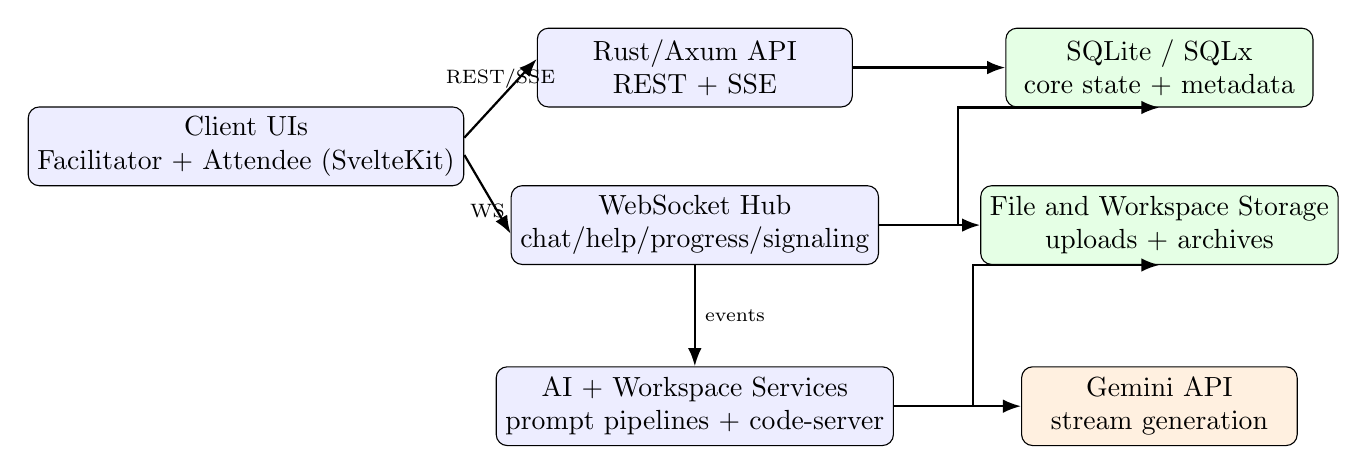
\begin{tikzpicture}[
  box/.style={draw, rounded corners, minimum width=40mm, minimum height=10mm, align=center, fill=blue!7},
  db/.style={draw, rounded corners, minimum width=39mm, minimum height=10mm, align=center, fill=green!10},
  ext/.style={draw, rounded corners, minimum width=35mm, minimum height=10mm, align=center, fill=orange!12},
  arrow/.style={-{Latex[length=2.3mm]}, thick}
]
\node[box] (client) at (0,0.8) {Client UIs\\Facilitator + Attendee (SvelteKit)};

\node[box] (api) at (5.7,1.8) {Rust/Axum API\\REST + SSE};
\node[box] (ws) at (5.7,-0.2) {WebSocket Hub\\chat/help/progress/signaling};
\node[box] (svc) at (5.7,-2.5) {AI + Workspace Services\\prompt pipelines + code-server};

\node[db] (db) at (11.6,1.8) {SQLite / SQLx\\core state + metadata};
\node[db] (fs) at (11.6,-0.2) {File and Workspace Storage\\uploads + archives};
\node[ext] (llm) at (11.6,-2.5) {Gemini API\\stream generation};

\draw[arrow] ([yshift=1.1mm]client.east) -- node[above, font=\scriptsize]{REST/SSE} ([yshift=1.1mm]api.west);
\draw[arrow] ([yshift=-1.1mm]client.east) -- node[below, font=\scriptsize]{WS} ([yshift=-1.1mm]ws.west);

\draw[arrow] (api.east) -- (db.west);
\draw[arrow] (ws.east) -- (fs.west);
\draw[arrow] (ws.east) -- ++(1.0,0) |- (db.south);
\draw[arrow] (ws.south) -- node[right, font=\scriptsize]{events} (svc.north);
\draw[arrow] (svc.east) -- (llm.west);
\draw[arrow] (svc.east) -- ++(1.0,0) |- (fs.south);
\end{tikzpicture}
}
}
}
\caption{Operational architecture used in Open Codelabs.}
\label{fig:system_architecture}
\end{figure}

\subsection{Live Session Signal Flow}
\begin{figure}[H]
\centering
\IfFileExists{figures/fig2-live-signal.pdf}{
\includegraphics[width=0.95\linewidth]{figures/fig2-live-signal.pdf}
}{
\IfFileExists{figures/fig2-live-signal.png}{
\includegraphics[width=0.95\linewidth]{figures/fig2-live-signal.png}
}{
\resizebox{0.95\linewidth}{!}{
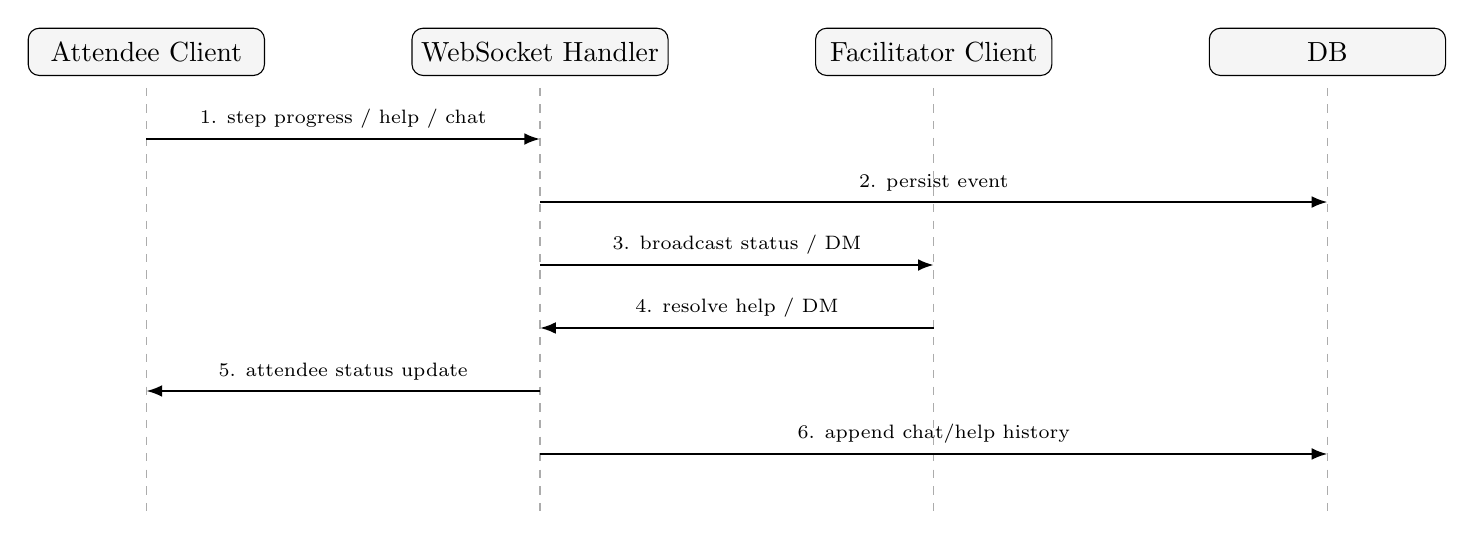
\begin{tikzpicture}[
  actor/.style={draw, minimum width=30mm, minimum height=6mm, fill=gray!8, rounded corners, align=center},
  lifeline/.style={gray!65, dashed, line width=0.45pt},
  msg/.style={-{Latex[length=2.0mm]}, thick},
  y=7.8mm
]
\node[actor] (att) at (0,0) {Attendee Client};
\node[actor] (ws) at (5.0,0) {WebSocket Handler};
\node[actor] (fac) at (10.0,0) {Facilitator Client};
\node[actor] (db) at (15.0,0) {DB};

\draw[lifeline] ([yshift=-1.5mm]att.south) -- ([yshift=-56mm]att.south);
\draw[lifeline] ([yshift=-1.5mm]ws.south) -- ([yshift=-56mm]ws.south);
\draw[lifeline] ([yshift=-1.5mm]fac.south) -- ([yshift=-56mm]fac.south);
\draw[lifeline] ([yshift=-1.5mm]db.south) -- ([yshift=-56mm]db.south);

\draw[msg] ([yshift=-8mm]att.south) -- node[midway, above, font=\scriptsize]{1. step progress / help / chat} ([yshift=-8mm]ws.south);
\draw[msg] ([yshift=-16mm]ws.south) -- node[midway, above, font=\scriptsize]{2. persist event} ([yshift=-16mm]db.south);
\draw[msg] ([yshift=-24mm]ws.south) -- node[midway, above, font=\scriptsize]{3. broadcast status / DM} ([yshift=-24mm]fac.south);
\draw[msg] ([yshift=-32mm]fac.south) -- node[midway, above, font=\scriptsize]{4. resolve help / DM} ([yshift=-32mm]ws.south);
\draw[msg] ([yshift=-40mm]ws.south) -- node[midway, above, font=\scriptsize]{5. attendee status update} ([yshift=-40mm]att.south);
\draw[msg] ([yshift=-48mm]ws.south) -- node[midway, above, font=\scriptsize]{6. append chat/help history} ([yshift=-48mm]db.south);
\end{tikzpicture}
}
}
}
\caption{Representative live classroom signal flow over WebSocket.}
\label{fig:ws_sequence}
\end{figure}

\subsection{Backend Control Surfaces}
Route assembly merges authentication, admin controls, codelab operations, uploads, AI services, WebSocket handling, and optional code-server endpoints into one router \cite{oc_routes}.
Core runtime configuration includes SQL migrations at startup and middleware stacks for rate limit, CSRF, and security headers \cite{oc_main_rs,oc_security_middleware}.

\subsection{Security and Governance Layers}
Security middleware explicitly configures CSP, HSTS, referrer policy, frame restrictions, and permission policy headers, with API-vs-static CSP branching \cite{oc_security_middleware}.
CSRF checks apply to state-changing methods when a session cookie is present, and rate limits are bucketed by route class (login, AI, upload, general) \cite{oc_security_middleware,oc_rate_limit}.
AI usage is also audit-recorded with actor and request metadata \cite{oc_ai_handler,oc_audit_tests}.

\section{Operational Protocols and Data Semantics}
\subsection{Facilitator Mode Surface Model}
The facilitator route is not a single-page editor with auxiliary dialogs; it is a multi-mode operational console.
The mode state in the admin codelab route exposes 15 explicit operational surfaces in one bounded workspace \cite{oc_guide_pipeline_component}.

\begin{table}[t]
\centering
\small
\caption{Facilitator operational modes and their dominant responsibilities.}
\label{tab:admin_modes}
\begin{tabular}{L{0.16\linewidth}L{0.27\linewidth}L{0.45\linewidth}}
\toprule
Mode & Primary intent & Representative actions \\
\midrule
edit & Authoring core content & Step markdown editing, inline AI improve, structural changes \\
preview & Render verification & Validate markdown/code rendering before release \\
guide & Preparation material pipeline & Standard or staged Pro guide generation, save and export \\
live & Classroom control & Monitor attendees, triage help queue, DM, announce \\
feedback & Outcome signal review & Difficulty/satisfaction review and qualitative comments \\
materials & Distribution control & Curate links/files and publish participant resources \\
quiz & Assessment authoring & Edit questions, run AI quiz generation, inspect submissions \\
submissions & Assignment review & Inspect uploaded files/links, remove invalid entries \\
gallery & Visual browsing & Session artifact inspection and image-oriented review \\
settings & Governance toggles & Completion requirements, visibility, metadata policies \\
workspace & Code-server management & Branch/folder snapshots, file edits, archive download \\
raffle & Completion-linked closeout & Participant raffle over verified completion pool \\
certificate & Credential lifecycle & Verify completion gates and certificate deliverability \\
ai & Consultant surface & Threaded facilitator advisory with optional grounding \\
monitoring & Ops telemetry & Session status observation and operational checks \\
\bottomrule
\end{tabular}
\end{table}

\subsection{WebSocket Contract Matrix}
The WebSocket channel carries heterogeneous event classes: collaboration, progress, and signaling.
Server logic enforces message-type-specific behavior (broadcast, direct fan-out, persistence side effects) \cite{oc_ws_handler}.

\small
\begin{longtable}{L{0.12\linewidth}L{0.16\linewidth}L{0.24\linewidth}L{0.32\linewidth}}
\caption{Live message contract matrix implemented in the WebSocket handler.}
\label{tab:ws_contract}\\
\toprule
Direction & Type & Required fields & Semantics \\
\midrule
\endfirsthead
\toprule
Direction & Type & Required fields & Semantics \\
\midrule
\endhead
\midrule
\multicolumn{4}{r}{Continued on next page} \\
\midrule
\endfoot
\bottomrule
\endlastfoot
Client $\rightarrow$ Server & chat & message & Persist chat row and broadcast to channel \\
Client $\rightarrow$ Server & dm & target\_id, message & Persist DM and fan-out to all target sessions \\
Client $\rightarrow$ Server & step\_progress & step\_number & Update attendee current step and broadcast progress \\
Client $\rightarrow$ Server & webrtc\_signal & signal (+ optional target\_id) & Direct or broadcast WebRTC signaling payload \\
Client $\rightarrow$ Server & screen\_share\_status & status & Update active facilitator-share map and broadcast status \\
Client $\rightarrow$ Server & attendee\_screen\_status & status & Update attendee share map and notify facilitator sessions \\
Server $\rightarrow$ Client & attendee\_joined & attendee object & Broadcast attendee arrival with current step snapshot \\
Server $\rightarrow$ Client & attendee\_left & attendee\_id & Broadcast departure when final tab/session closes \\
Server $\rightarrow$ Client & screen\_share\_status & sender\_id, status & Class-wide facilitator share state updates \\
Server $\rightarrow$ Client & attendee\_screen\_status & attendee\_id, attendee\_name, status & Facilitator visibility into attendee share participation \\
Server $\rightarrow$ Client & dm/chat/step\_progress & message-specific payload & Delivery for persisted communication/progress events \\
\end{longtable}
\normalsize

\subsection{Data Invariants and Completion Gate Semantics}
The schema and handler behavior imply explicit invariants beyond simple CRUD \cite{oc_db_schema_doc,oc_routes,oc_ai_handler}.
Representative invariants include:
\begin{itemize}[leftmargin=1.2em]
  \item at most one workspace row per codelab (\texttt{codeserver\_workspaces.codelab\_id} is unique),
  \item inline comment thread uniqueness per anchor key within a codelab,
  \item codelab-scoped ownership checks for attendee submissions and AI conversation writes,
  \item thread ownership enforcement for facilitator consultant message access.
\end{itemize}

Completion is controlled by requirement toggles (quiz, feedback, submission).
For attendee $i$ in codelab $c$, define:
\begin{equation}
G_{i,c}=\mathbf{1}\!\left(
q_c\Rightarrow Q_{i,c}
\right)
\mathbf{1}\!\left(
f_c\Rightarrow F_{i,c}
\right)
\mathbf{1}\!\left(
s_c\Rightarrow S_{i,c}
\right),
\label{eq:gate}
\end{equation}
where $q_c,f_c,s_c\in\{0,1\}$ are codelab requirement toggles and $Q_{i,c},F_{i,c},S_{i,c}\in\{0,1\}$ are attendee fulfillment states.
Certificate eligibility is satisfied when $G_{i,c}=1$.

\subsection{Migration and Compatibility Strategy}
The backend migration history records iterative expansion from core codelab tables to real-time support, assessment, workspace orchestration, AI thread persistence, and inline comments \cite{oc_db_schema_doc}.
This evolution pattern matters operationally:
\begin{itemize}[leftmargin=1.2em]
  \item feature introduction is append-only at schema level where possible,
  \item compatibility risk is concentrated around columns that alter completion or message semantics,
  \item workshop operators can reason about rollout order from migration timestamps.
\end{itemize}

\section{AI Subsystem: Design and Operations}
\subsection{AI Surface Inventory}
Open Codelabs exposes five distinct AI surfaces:
\begin{itemize}[leftmargin=1.2em]
  \item AI Codelab Generator (basic/prompt-only/advanced staged generation).
  \item Preparation Guide Generator (single-pass and Pro staged flow).
  \item Facilitator Consultant (threaded multi-turn advisory chat with search grounding).
  \item Ask Gemini (attendee-side contextual Q\&A).
  \item AI quiz generation and inline markdown improvement.
\end{itemize}
These surfaces share a common transport and telemetry substrate but use different prompt templates and output contracts \cite{oc_ai_generator_component,oc_guide_pipeline_component,oc_consultant_component,oc_ask_gemini_component,oc_gemini_client}.

\subsection{AI Codelab Generator Pipeline}
The codelab generator implements three operating modes:
\begin{itemize}[leftmargin=1.2em]
  \item \textbf{Basic mode:} one-pass structured generation into title/description/steps JSON.
  \item \textbf{Prompt-only mode:} tutorial steps constrained to prompt-centric pedagogy without mandatory code emission.
  \item \textbf{Advanced staged mode:} plan $\rightarrow$ draft $\rightarrow$ third-party style review $\rightarrow$ revision.
\end{itemize}
Advanced mode is especially relevant for production workshops because it separates structural planning from narrative synthesis and introduces an explicit review checkpoint before final output application \cite{oc_ai_generator_component}.
The staged protocol also allows optional Google Search grounding and facilitator comment injection into draft prompts.

\subsection{Gemini Pro Mode: Agentic Workflow for Codelab Synthesis}
The Gemini-based Pro mode is implemented as an explicit stateful, multi-agent pipeline rather than a single prompt.
In implementation terms, the frontend tracks explicit stage labels:
\texttt{input -> planning -> plan -> drafting -> draft -> reviewing -> revising -> final}.
Planner, drafter, reviewer, and reviser are separated by schema boundaries (plan JSON, draft JSON, review JSON, revised JSON), and each transition is conditioned on structured-output parse success \cite{oc_ai_generator_component,oc_gemini_client}.
When parsing fails, the controller falls back to the nearest safe upstream stage (for example, draft parse failure returns to plan; review/revise parse failure returns to draft) instead of auto-publishing partial output.

Pro mode separates artifact roles as follows:
\begin{itemize}[leftmargin=1.2em]
  \item \textbf{Plan agent:} emits objectives, prerequisites, environment setup, per-step verification, and \texttt{search\_terms}.
  \item \textbf{Draft agent:} converts plan + source context (+ facilitator comments) into tutorial markdown JSON.
  \item \textbf{Review agent:} audits structural and pedagogical defects and emits actionable issue list.
  \item \textbf{Revise agent:} applies review output and finalizes publishable codelab content.
\end{itemize}

\begin{table}[t]
\centering
\small
\caption{Pro-mode agent stage contracts in Gemini codelab generation.}
\label{tab:pro_agent_contract}
\begin{tabular}{L{0.14\linewidth}L{0.16\linewidth}L{0.28\linewidth}L{0.18\linewidth}L{0.16\linewidth}}
\toprule
Stage & Agent role & Output contract & Tool access & Fallback on parse fail \\
\midrule
Planning & Planner & Plan JSON (audience, objectives, env setup, step goals, \texttt{search\_terms}) & none & \texttt{input} \\
Drafting & Drafter & Codelab JSON (title/description/steps) & optional \texttt{googleSearch}, optional \texttt{urlContext} & \texttt{plan} \\
Reviewing & Reviewer & Review JSON (summary, issues, missing items, improvements) & none & \texttt{draft} \\
Revising & Reviser & Revised codelab JSON (publishable) & optional \texttt{googleSearch}, optional \texttt{urlContext} & \texttt{draft} \\
\bottomrule
\end{tabular}
\end{table}

The landing page publicly exposes the same conceptual graph (Inputs $\rightarrow$ Plan $\rightarrow$ Draft $\rightarrow$ Review $\rightarrow$ Revise $\rightarrow$ Final, with query-grounding side loop), and this aligns with implementation states and tool routing \cite{oc_landing_page,oc_ai_generator_component}.

\begin{figure}[t]
\centering
\resizebox{0.99\linewidth}{!}{
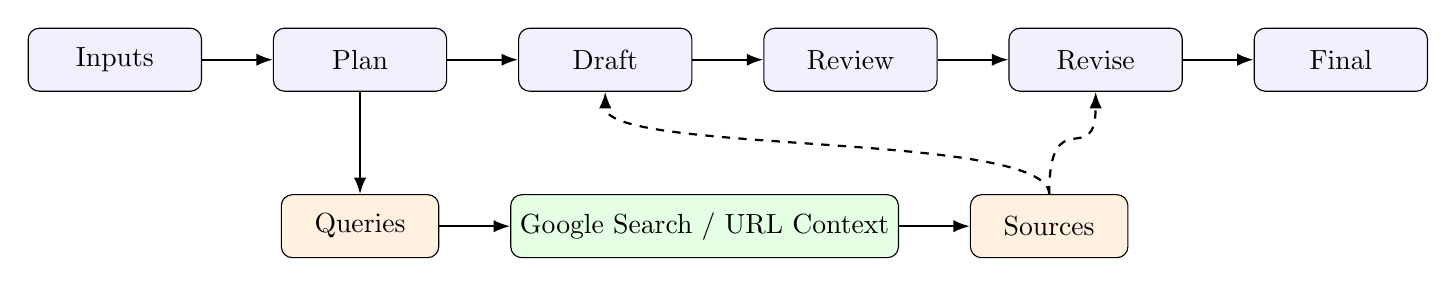
\begin{tikzpicture}[
  node distance=8mm and 9mm,
  nodebox/.style={draw, rounded corners, minimum width=22mm, minimum height=8mm, align=center, fill=blue!6},
  toolbox/.style={draw, rounded corners, minimum width=26mm, minimum height=8mm, align=center, fill=green!10},
  auxbox/.style={draw, rounded corners, minimum width=20mm, minimum height=8mm, align=center, fill=orange!12},
  flow/.style={-{Latex[length=2.1mm]}, thick}
]
\node[nodebox] (in) {Inputs};
\node[nodebox, right=of in] (plan) {Plan};
\node[nodebox, right=of plan] (draft) {Draft};
\node[nodebox, right=of draft] (review) {Review};
\node[nodebox, right=of review] (revise) {Revise};
\node[nodebox, right=of revise] (final) {Final};

\node[auxbox, below=13mm of plan] (queries) {Queries};
\node[toolbox, right=of queries] (gsearch) {Google Search / URL Context};
\node[auxbox, right=of gsearch] (sources) {Sources};

\draw[flow] (in) -- (plan);
\draw[flow] (plan) -- (draft);
\draw[flow] (draft) -- (review);
\draw[flow] (review) -- (revise);
\draw[flow] (revise) -- (final);

\draw[flow] (plan) -- (queries);
\draw[flow] (queries) -- (gsearch);
\draw[flow] (gsearch) -- (sources);
\draw[flow, dashed] (sources.north) .. controls +(0,8mm) and +(0,-8mm) .. (draft.south);
\draw[flow, dashed] (sources.north) .. controls +(0,12mm) and +(0,-10mm) .. (revise.south);
\end{tikzpicture}
}
\caption{Gemini Pro-mode agent workflow and grounding-tool side loop for codelab generation.}
\label{fig:pro_agent_workflow}
\end{figure}

\subsection{AI Agent Tool Inventory and Exposure Boundaries}
Tool availability is not uniform across AI surfaces.
The implementation-level rule is flow- and stage-specific allowlisting over \texttt{googleSearch}, \texttt{urlContext}, and transport-exposed tool payloads.
This avoids conflating ``AI enabled'' with ``all tools enabled'' and keeps authority boundaries explicit per workflow stage.

\begin{table}[t]
\centering
\small
\caption{AI-agent tool exposure by product flow and implementation layer.}
\label{tab:agent_tool_inventory}
\begin{tabular}{L{0.22\linewidth}L{0.20\linewidth}L{0.20\linewidth}L{0.22\linewidth}}
\toprule
Flow & Model path & Exposed tools & Notes \\
\midrule
AI Codelab Generator (Pro draft/revise) & \texttt{streamGeminiStructuredOutput} & optional \texttt{googleSearch}, optional \texttt{urlContext} & Planner/reviewer run without tools; toggles controlled in UI \\
Preparation Guide (Pro draft/revise) & \texttt{streamGeminiStructuredOutput} & \texttt{googleSearch} & Plan/review stages run without tool payload \\
Facilitator Consultant & \texttt{streamGeminiChat} & \texttt{googleSearch} & Grounding metadata persisted to thread messages \\
Ask Gemini attendee Q\&A & \texttt{streamGeminiResponseRobust} & none (default) & Context-question wrapper, no explicit grounding tool injection \\
Backend AI proxy contract & \path{/api/ai/stream} & pass-through JSON \texttt{tools} & Transport accepts arbitrary tool JSON; integration test includes \texttt{codeExecution} payload \\
\bottomrule
\end{tabular}
\end{table}

The practical implication is that ``agent'' in Open Codelabs is a staged orchestration pattern over multiple Gemini calls with selective tool activation, not a single monolithic black-box response \cite{oc_ai_generator_component,oc_guide_pipeline_component,oc_consultant_component,oc_ask_gemini_component,oc_gemini_client,oc_ai_handler,oc_api_tests}.

\subsection{Preparation Guide Generation Pipeline}
Guide generation is implemented twice: a standard direct pass and a Pro staged pass.
The Pro variant builds a plan JSON (summary, audience, prerequisites, sections, checklist, search terms), drafts markdown, performs dual-perspective review (expert + novice), and revises accordingly \cite{oc_guide_pipeline_component}.
This design reduces one-pass hallucination risk by enforcing intermediate structured artifacts.

Input context is bounded by prompt-budget guards (\texttt{MAX\_GUIDE\_PROMPT\_CHARS}, per-step truncation, section-level truncation notes), which makes generation predictable under large codelab payloads while preserving explicit truncation transparency for the operator.

\subsection{Consultant and Attendee Q\&A Flows}
Facilitator Consultant uses multi-turn thread persistence with optional grounding metadata capture; attendee Ask-Gemini uses step-contextual question answering with optional conversation persistence.
These two flows share transport primitives but differ in governance:
\begin{itemize}[leftmargin=1.2em]
  \item facilitator flow is thread-centric and admin-scoped,
  \item attendee flow is codelab-bound and participant-scoped,
  \item both parse usage metadata for token accounting.
\end{itemize}
This split allows high-agency facilitator ideation without overloading attendee UI with workflow complexity \cite{oc_consultant_component,oc_ask_gemini_component,oc_ai_handler}.

\subsection{AI Safety and Governance Controls}
The AI proxy enforces prompt validation, role-aware codelab scoping, model-name validation (including optional allow-list environment policy), encrypted API-key forwarding, and audit logging \cite{oc_ai_handler}.
From an operations perspective, this establishes a governance boundary:
\begin{itemize}[leftmargin=1.2em]
  \item frontend templates remain inspectable and version-controlled,
  \item backend enforces policy and persistence constraints,
  \item per-request metadata supports retrospective incident analysis.
\end{itemize}

\subsection{Transport and Contract Model}
The Gemini client helper supports three transport forms:
\begin{itemize}[leftmargin=1.2em]
  \item \texttt{streamGeminiResponseRobust}: context-question wrapper text payload.
  \item \texttt{streamGeminiChat}: role-normalized chat messages with optional \texttt{system\_instruction}.
  \item \texttt{streamGeminiStructuredOutput}: schema-constrained JSON output with optional thinking-level config.
\end{itemize}
For backend mode, payloads are proxied through \path{/api/ai/stream} with encrypted API key forwarding and CSRF headers \cite{oc_gemini_client,oc_ai_handler}.

\subsection{Model Inventory and Effective Selection Rules}
The implementation uses a single dominant runtime model family in production code paths: \texttt{gemini-3-flash-preview}.
This appears both as the frontend default and backend proxy fallback when \texttt{model} is omitted \cite{oc_gemini_client,oc_ai_handler}.

\begin{table}[t]
\centering
\small
\caption{Model usage inventory by AI surface (implementation-level).}
\label{tab:model_inventory}
\begin{tabular}{L{0.20\linewidth}L{0.26\linewidth}L{0.16\linewidth}L{0.22\linewidth}}
\toprule
Surface & Request assembly path & Effective runtime model & Notes \\
\midrule
Ask Gemini (attendee) & \path{AskGemini.svelte -> streamGeminiResponseRobust} & Default \texttt{gemini-3-flash-preview} & Saved label may remain \texttt{gemini-1.5-flash} \\
Facilitator Consultant & \path{FacilitatorConsultant.svelte -> streamGeminiChat} & Explicit \texttt{gemini-3-flash-preview} & Uses \texttt{googleSearch} tool option \\
AI Codelab Generator & \path{AiCodelabGenerator.svelte -> structured stream} & Explicit \texttt{gemini-3-flash-preview} & Supports high thinking level and optional tools \\
Guide generation (admin page) & \path{admin/[id]/+page.svelte helper path} & Explicit \texttt{gemini-3-flash-preview} & Includes staged plan/draft/review/revise variants \\
Backend proxy fallback & \path{proxy_gemini_stream (AI handler)} & Default \texttt{gemini-3-flash-preview} & Applied when request model is absent \\
\bottomrule
\end{tabular}
\end{table}

Runtime model resolution follows three concrete branches:
\begin{itemize}[leftmargin=1.2em]
  \item use request model when present and valid under allow-list/policy checks;
  \item use backend default (\texttt{gemini-3-flash-preview}) when absent;
  \item reject invalid model names before upstream calls.
\end{itemize}
For auditing, persisted conversation labels are compared against runtime model usage.
In the attendee Ask-Gemini path, a mismatch can appear because persistence still stores a legacy label (\texttt{gemini-1.5-flash}) while runtime defaults to \texttt{gemini-3-flash-preview} unless overridden \cite{oc_ask_gemini_component,oc_gemini_client,oc_ai_handler}.

\subsection{External AI API and Tool Capability Matrix}
Open Codelabs uses the Gemini streaming generation endpoint with both direct (serverless mode) and proxied (backend mode) transport.
The implementation exposes advanced capability knobs rather than a minimal text-only call surface.

\begin{table}[t]
\centering
\small
\caption{External AI API capability contracts used by the system.}
\label{tab:ai_api_contract}
\begin{tabular}{L{0.23\linewidth}L{0.27\linewidth}L{0.42\linewidth}}
\toprule
Capability & Contract field / endpoint & Implementation behavior \\
\midrule
Streaming generation & \path{/v1beta/models/\{model\}:streamGenerateContent?alt=sse} & Parses SSE \texttt{data:} events and incremental text chunks \\
Role-based chat transport & \texttt{contents[role,parts]} + optional \texttt{system\_instruction} & Normalizes assistant role to Gemini \texttt{model} role \\
Structured JSON output & \path{generationConfig.responseMimeType=application/json}, \path{responseJsonSchema} & Enforces schema-constrained generation for codelab/guide pipelines \\
Reasoning budget control & \path{generationConfig.thinkingConfig.thinkingLevel} & Supports low/medium/high thinking level selection \\
Grounding tools & \path{tools=[{googleSearch},{urlContext}]} & Selective tool activation per feature flow \\
Governed backend proxy & \path{/api/ai/stream} & Adds auth/CSRF enforcement, prompt validation, audit metadata, and key handling \\
\bottomrule
\end{tabular}
\end{table}

\subsection{Prompt Governance and Transparency}
Prompt logic is not hidden in backend binaries; it is declared in frontend components and sent through explicit API payload fields.
This provides versionable, reviewable prompt evolution at the source level.
To align with transparent research reporting, this report publishes all system-level prompt templates in \cref{app:prompts}.
For verbatim implementation excerpts with prompt-construction logic and payload assembly, see \cref{app:prompt_sources}.

\subsection{AI Cost and Latency Observability}
Token usage metadata is parsed from stream events and persisted in conversation/thread records, enabling direct cost accounting and retrospective auditing \cite{oc_gemini_client,oc_ai_handler}.
Grounding metadata from search-enabled responses is also retained in consultant/thread flows for source traceability \cite{oc_consultant_component,oc_ai_handler}.

\section{API and Deployment Datasheet}
\subsection{Route-Level Availability Summary}
The backend router currently declares 55 distinct API paths and 69 method-path operations.
This difference is expected because several paths expose multiple methods (for example GET+POST or GET+PUT+DELETE) \cite{oc_routes}.
Main route catalog is listed in \cref{app:api}; reproducibility-oriented router/DTO/domain source anchors and regeneration commands are provided in \cref{app:api_datasheet}.

\begin{table}[t]
\centering
\small
\caption{Route families and declared path counts.}
\label{tab:route_family_counts}
\begin{tabular}{L{0.30\linewidth}C{0.16\linewidth}L{0.45\linewidth}}
\toprule
Route family & Distinct paths & Scope \\
\midrule
Authentication & 3 & Login, logout, session \\
Admin governance & 6 & Settings, updates, audit, backup export/inspect/restore \\
Codelab domain + certificates & 28 & Lifecycle, attendees, help, feedback, quizzes, submissions, comments, chat, AI conversation list \\
Upload & 2 & Image and material file upload \\
AI core & 4 & Stream proxy, conversation save, thread CRUD/message \\
WebSocket & 1 & Session channel endpoint \\
Code-server workspace & 11 & Workspace lifecycle, branch/folder operations, archive/download \\
\midrule
Total & 55 & Path-level declarations in router \\
\bottomrule
\end{tabular}
\end{table}

\begin{table}[t]
\centering
\small
\caption{HTTP method distribution over declared API operations.}
\label{tab:method_mix}
\begin{tabular}{L{0.28\linewidth}C{0.20\linewidth}L{0.40\linewidth}}
\toprule
Method & Count & Typical usage class \\
\midrule
GET & 30 & Read/list/query operations, WebSocket upgrade endpoint \\
POST & 30 & Create/mutate actions, AI streaming trigger, uploads \\
PUT & 3 & Bulk update and idempotent codelab/quiz writes \\
DELETE & 6 & Resource deletion and cleanup \\
\midrule
Total & 69 & Method-path operation count \\
\bottomrule
\end{tabular}
\end{table}

\subsection{Frontend API Abstraction and Multi-Backend Modes}
The frontend exposes one API facade that dispatches by runtime mode:
\texttt{backend}, \texttt{firebase}, or \texttt{supabase}.
Mode is selected by build-time flags (\texttt{VITE\_USE\_FIREBASE}, \texttt{VITE\_USE\_SUPABASE}) and some operations intentionally degrade to no-op, empty-list, or explicit not-supported errors in serverless paths \cite{oc_frontend_api_selector}.

\begin{table}[t]
\centering
\small
\caption{Capability compatibility across frontend API modes.}
\label{tab:mode_compat}
\begin{tabular}{L{0.36\linewidth}C{0.16\linewidth}C{0.16\linewidth}C{0.16\linewidth}}
\toprule
Capability cluster & backend mode & firebase mode & supabase mode \\
\midrule
Core codelab CRUD and attendee registration & Full & Full & Full \\
Code-server workspace operations & Full & Not supported & Not supported \\
Backup inspect/restore and codelab import/export & Full & Not supported & Not supported \\
Material/submission/quiz admin flows & Full & Partial/limited & Mostly full \\
AI conversation persistence/list retrieval & Full & save no-op/list empty & save no-op/list empty \\
Auth provider switching (Google login) & Not supported & Supported & Supported \\
\bottomrule
\end{tabular}
\end{table}

\subsection{Build Footprint and Minimum System Specification}
To make deployment planning concrete, we measured artifact sizes in the current repository workspace after production-style builds (\texttt{cargo build --release --bin backend}, \texttt{bun run build}) and Docker image inspection on the same host.
Table values are implementation-grounded measurements, not theoretical estimates.

\begin{table}[t]
\centering
\scriptsize
\caption{Measured storage footprint of key build and deployment artifacts (2026-02-19 snapshot).}
\label{tab:build_footprint}
\begin{tabular}{L{0.27\linewidth}L{0.11\linewidth}L{0.50\linewidth}}
\toprule
Artifact & Size & Measurement context \\
\midrule
Backend release service binary (\texttt{target/release/backend}) & 23 MB & Native arm64 release binary \\
Frontend production bundle (\texttt{frontend/build}) & 14 MB & SvelteKit adapter-bun output \\
Frontend client output only (\texttt{.svelte-kit/output/client}) & 6.4 MB & Static client payload subset \\
Frontend server output only (\texttt{.svelte-kit/output/server}) & 3.0 MB & SSR/server chunks subset \\
Local frontend dependencies (\texttt{frontend/node\_modules}) & 505 MB & Developer machine dependency cache \\
Local backend release target tree (\texttt{backend/target/release}) & 1.0 GB & Includes binary + Rust build artifacts \\
Backend data directory (\texttt{backend/data}) & 1.0 MB & Local snapshot (workload/content dependent; includes active SQLite files) \\
Docker image: \texttt{open-codelabs-frontend} & 536 MB & Local image store (\texttt{docker images}) \\
Docker image: \texttt{open-codelabs-backend} & 234 MB & Local image store (\texttt{docker images}) \\
\bottomrule
\end{tabular}
\end{table}

For capacity planning, operators should split storage into three practical buckets:
runtime images, build/dependency cache, and time-varying data/log volumes.
Using measured images, the base container footprint is approximately $536 + 234 = 770$ MB before persistent data and logs.

\begin{table}[t]
\centering
\small
\caption{Minimum system specification and operational baseline.}
\label{tab:min_spec}
\begin{tabular}{L{0.28\linewidth}L{0.26\linewidth}L{0.38\linewidth}}
\toprule
Profile & Requirement & Notes \\
\midrule
Documented minimum & 2 GB RAM, 1 GB free disk, Linux/macOS/Windows(WSL2) & Official installation baseline \cite{oc_installation_en_doc} \\
Software baseline (Docker path) & Docker Engine 20.10+, Docker Compose v2.0+ & Recommended installation path \cite{oc_installation_en_doc,open_codelabs_readme} \\
Software baseline (local dev path) & Rust 1.75+, Bun 1.0+, SQLite 3.35+ & Native development path \cite{oc_installation_en_doc} \\
Observed practical disk baseline (Docker) & $\ge$ 3 GB free recommended & Inference from 770 MB image footprint + DB/log/backup headroom \\
Load-tested concurrency evidence & 100 stable, 200 maximum-tested users & FAQ operational report; CPU rises near upper bound \cite{oc_faq_en_doc} \\
\bottomrule
\end{tabular}
\end{table}

Because workshop data grows with attendee submissions, chat/help history, and uploaded materials, operators should track persistent data/log growth over time rather than relying only on static image size.

\subsection{API Contract Transparency and Reproducibility}
To make this report auditable as a systems artifact rather than a marketing summary, API evidence is disclosed at multiple layers:
\begin{itemize}[leftmargin=1.2em]
  \item route registration source (\texttt{routes.rs}),
  \item DTO payload contracts used by handlers,
  \item domain model structs for persisted records,
  \item published API reference document with request/response examples.
\end{itemize}
These are indexed with representative excerpts and reproducible counting commands in \cref{app:api_datasheet}, and cross-checkable against the endpoint catalog in \cref{app:api} \cite{oc_routes,oc_api_reference_doc}.

\FloatBarrier
\section{Database Architecture and Data Datasheet}
\subsection{Schema Evolution and Integrity Inventory}
Database behavior is migration-driven through \texttt{backend/migrations} and applied at startup using \texttt{sqlx::migrate!}.
In current repository state, the migration corpus contains 26 files with 17 table-creation statements and 21 schema-alteration statements \cite{oc_migrations_dir,oc_main_rs}.
The schema includes 19 explicit non-comment foreign-key clauses and 10 index definitions (9 \texttt{CREATE INDEX} + 1 \texttt{CREATE UNIQUE INDEX}), plus 3 \texttt{UNIQUE} constraints at table/column definition level across operational domains (learning flow, realtime, AI metadata, workspace, and audit).

\begin{table}[t]
\centering
\small
\caption{Database structure metrics from migration corpus.}
\label{tab:db_structure_metrics}
\begin{tabular}{L{0.48\linewidth}C{0.16\linewidth}L{0.28\linewidth}}
\toprule
Metric & Value & Interpretation \\
\midrule
Migration files & 26 & Sequential schema evolution history \\
CREATE TABLE statements & 17 & Logical relation count at DDL level \\
ALTER TABLE statements & 21 & Incremental evolution pressure on existing entities \\
Foreign-key clauses & 19 & Referential constraints for codelab-scoped integrity \\
Index definitions (\texttt{CREATE INDEX}/\texttt{CREATE UNIQUE INDEX}) & 10 & Query acceleration paths over hot access patterns \\
\texttt{UNIQUE} constraints (table/column) & 3 & Declarative integrity constraints for key tuple/value uniqueness \\
Data backfill UPDATE statements & 1 & Explicit historical field migration (\texttt{correct\_answers}) \\
\bottomrule
\end{tabular}
\end{table}

\subsection{ER Diagram of Runtime Schema}
\begin{figure}[t]
\centering
\resizebox{0.98\linewidth}{!}{
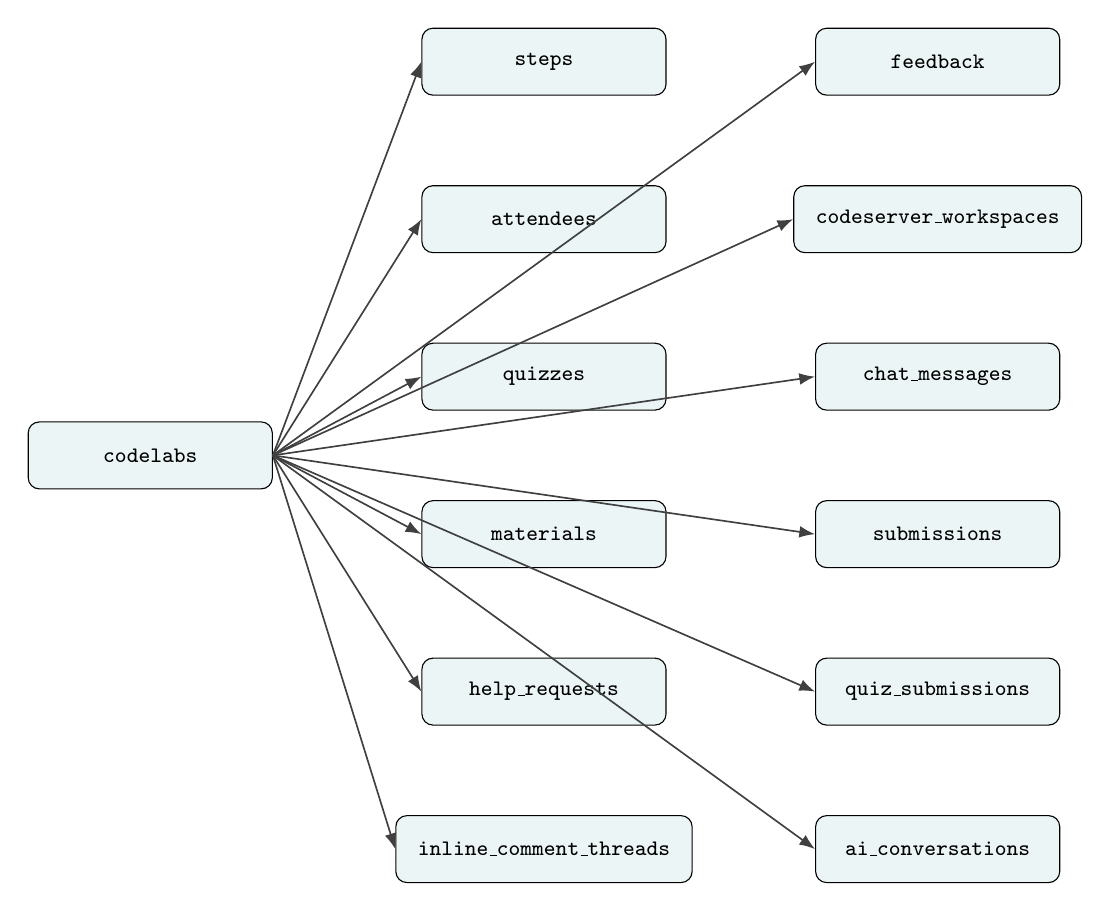
\begin{tikzpicture}[
  x=1.0cm, y=1.0cm,
  tbl/.style={draw, rounded corners, minimum height=8.5mm, minimum width=31mm, inner xsep=2.8mm, align=center, fill=teal!8, font=\footnotesize},
  edge/.style={-{Latex[length=2.0mm]}, semithick, draw=black!75}
]
\node[tbl] (codelabs) at (-5.0,0.0) {\texttt{codelabs}};

\node[tbl] (steps) at (0.0,5.0) {\texttt{steps}};
\node[tbl] (attendees) at (0.0,3.0) {\texttt{attendees}};
\node[tbl] (quizzes) at (0.0,1.0) {\texttt{quizzes}};
\node[tbl] (materials) at (0.0,-1.0) {\texttt{materials}};
\node[tbl] (help) at (0.0,-3.0) {\texttt{help\_requests}};
\node[tbl] (inline_t) at (0.0,-5.0) {\texttt{inline\_comment\_threads}};

\node[tbl] (feedback) at (5.0,5.0) {\texttt{feedback}};
\node[tbl] (cs) at (5.0,3.0) {\texttt{codeserver\_workspaces}};
\node[tbl] (chat) at (5.0,1.0) {\texttt{chat\_messages}};
\node[tbl] (submissions) at (5.0,-1.0) {\texttt{submissions}};
\node[tbl] (quiz_sub) at (5.0,-3.0) {\texttt{quiz\_submissions}};
\node[tbl] (ai_conv) at (5.0,-5.0) {\texttt{ai\_conversations}};

\draw[edge] (codelabs.east) -- (steps.west);
\draw[edge] (codelabs.east) -- (attendees.west);
\draw[edge] (codelabs.east) -- (quizzes.west);
\draw[edge] (codelabs.east) -- (materials.west);
\draw[edge] (codelabs.east) -- (help.west);
\draw[edge] (codelabs.east) -- (inline_t.west);
\draw[edge] (codelabs.east) -- (feedback.west);
\draw[edge] (codelabs.east) -- (cs.west);
\draw[edge] (codelabs.east) -- (chat.west);
\draw[edge] (codelabs.east) -- (submissions.west);
\draw[edge] (codelabs.east) -- (quiz_sub.west);
\draw[edge] (codelabs.east) -- (ai_conv.west);
\end{tikzpicture}
}
\caption{Core database structure derived from migration DDL (first-order codelab-scoped foreign keys).}
\label{fig:db_erd}
\end{figure}

\begin{table}[t]
\centering
\small
\caption{Secondary explicit and contextual links separated from \cref{fig:db_erd} for readability.}
\label{tab:db_secondary_links}
\begin{tabular}{L{0.30\linewidth}L{0.60\linewidth}}
\toprule
Link class & Relations \\
\midrule
Secondary explicit FK & \texttt{attendees -> help\_requests}, \texttt{attendees -> feedback}, \texttt{attendees -> submissions}, \texttt{attendees -> quiz\_submissions}, \texttt{quizzes -> quiz\_submissions}, \texttt{inline\_comment\_threads -> inline\_comment\_messages}, \texttt{ai\_threads -> ai\_messages} \\
Contextual/optional linkage & \texttt{ai\_threads -> codelabs}, \texttt{audit\_logs -> codelabs} \\
\bottomrule
\end{tabular}
\end{table}

\subsection{DML Workload Semantics}
The backend handler/audit layer embeds a large SQL DML surface with query classes spanning read models, command writes, event logging, and backup restore workflows.
A source-line keyword inventory over SQL-bearing lines in \texttt{backend/src/api/handlers} and \texttt{backend/src/infrastructure/audit.rs} yields 93 \texttt{SELECT}, 47 \texttt{INSERT INTO}, 10 \texttt{UPDATE}, and 44 \texttt{DELETE FROM} occurrences in the current snapshot \cite{oc_db_dml_queries}.

\begin{table}[t]
\centering
\small
\caption{DML class distribution across handler and audit SQL-bearing lines.}
\label{tab:dml_mix}
\begin{tabular}{L{0.30\linewidth}C{0.16\linewidth}L{0.44\linewidth}}
\toprule
DML class & Count & Dominant use pattern \\
\midrule
\texttt{SELECT} & 93 & codelab/attendee/material/AI retrieval and admin analytics views \\
\texttt{INSERT INTO} & 47 & attendee events, AI/chat persistence, backup restore writes \\
\texttt{UPDATE} & 10 & progress, resolution, status evolution, and timestamp transitions \\
\texttt{DELETE FROM} & 44 & lifecycle cleanup, codelab deletion cascade orchestration, and backup reset paths \\
\bottomrule
\end{tabular}
\end{table}

\subsection{Schema Datasheet Synchronization Status}
To avoid documentation drift in this revised manuscript, all database metrics reported here and in \cref{app:db_datasheet} are regenerated directly from migration files at the manuscript snapshot commit (\texttt{a3510b39}) rather than copied from prose documentation.
The public schema document remains useful as a conceptual reference, but migration SQL is treated as source-of-truth for reproducible counting and integrity analysis.
To keep this report auditable while maintaining manuscript conciseness, \cref{app:db_datasheet} provides source anchors, representative DDL excerpts, and exact regeneration commands for all reported metrics.

\section{Security Architecture and Cryptographic Protocols}
\subsection{Threat Model and Control Objectives}
Open Codelabs is exposed as a stateful web system with authenticated facilitator and attendee sessions, cross-origin browser traffic, WebSocket channels, file uploads, and external AI API interactions.
The primary security objectives are:
\begin{itemize}[leftmargin=1.2em]
  \item prevent unauthorized state changes (auth + CSRF + role checks),
  \item protect sensitive fields (attendee join codes, admin-provided AI keys),
  \item bound abusive traffic (bucketed rate limits),
  \item preserve forensic visibility (audit event capture with request metadata).
\end{itemize}

\subsection{Defense-in-Depth Control Inventory}
\begin{table}[t]
\centering
\small
\caption{Security control layers and concrete enforcement points.}
\label{tab:security_controls}
\begin{tabular}{L{0.24\linewidth}L{0.28\linewidth}L{0.40\linewidth}}
\toprule
Control family & Mechanism & Implementation anchors \\
\midrule
Session auth & JWT (HS256) with issuer/audience validation, cookie-scoped sessions & \texttt{auth.rs}, login/register handlers \cite{oc_auth_middleware,oc_admin_handler,oc_attendees_handler} \\
CSRF defense & Double-submit cookie validation for unsafe methods (\texttt{X-CSRF-Token}) & \texttt{csrf\_middleware}, frontend CSRF header propagation \cite{oc_security_middleware,oc_api_backend_client,oc_api_reference_doc} \\
Header hardening & CSP, HSTS(HTTPS), X-Frame-Options, nosniff, referrer-policy, permissions-policy & Backend security middleware + frontend hook fallback \cite{oc_security_middleware,oc_frontend_hooks} \\
Abuse control & Route-class bucket rate limiting (login/AI/upload/general) by client key & \texttt{rate\_limit.rs}, middleware classifier \cite{oc_rate_limit,oc_security_middleware} \\
Secret protection & Password-based encryption with integrity tag and constant-time verification & \texttt{utils/crypto.rs}, client encryption helper \cite{oc_backend_crypto,oc_frontend_crypto} \\
Auditability & Append-oriented audit event recording in normal operations (with backup-restore rewrite path) & Audit infra + admin retrieval route \cite{oc_audit_tests,oc_routes} \\
\bottomrule
\end{tabular}
\end{table}

\subsection{Cryptographic Construction for Sensitive Fields}
Backend-side secret protection is implemented with a password-based envelope:
PBKDF2-HMAC-SHA256 key derivation, AES-256-CBC encryption with PKCS\#7 padding, and HMAC-SHA256 authentication over payload bytes.
The ciphertext format is versioned as \texttt{v1:BASE64(salt || iv || ciphertext || tag)} \cite{oc_backend_crypto}.
This construction is used for attendee code storage and for encrypted admin AI-key transport validation \cite{oc_attendees_handler,oc_admin_handler}.

\begin{table}[t]
\centering
\small
\caption{Cryptographic parameters used by backend encryption utility.}
\label{tab:crypto_params}
\begin{tabular}{L{0.42\linewidth}L{0.20\linewidth}L{0.28\linewidth}}
\toprule
Parameter & Value & Role \\
\midrule
PBKDF2 iteration count $r$ & 100,000 & Password stretching cost factor \\
Salt length $|S|$ & 16 bytes & Per-message randomness for key derivation \\
IV length $|IV|$ & 16 bytes & CBC nonce/initialization vector \\
Derived key material & 64 bytes & Split into $K_{enc}$ and $K_{mac}$ \\
Encryption key $|K_{enc}|$ & 32 bytes & AES-256-CBC key \\
MAC key $|K_{mac}|$ & 32 bytes & HMAC-SHA256 key \\
Tag length $|T|$ & 32 bytes & Integrity/authentication tag \\
\bottomrule
\end{tabular}
\end{table}

Let password be $P$, salt $S$, plaintext $M$, and random IV be $IV$.
Key derivation is:
\begin{equation}
(K_{enc}\|K_{mac})=\mathrm{PBKDF2}_{\mathrm{HMAC\mbox{-}SHA256}}(P,S,r,64),\quad r=100000.
\label{eq:kdf}
\end{equation}
Encryption and authentication are:
\begin{equation}
C=\mathrm{AES\mbox{-}256\mbox{-}CBC}^{\mathrm{PKCS7}}_{K_{enc}}(IV,M),\qquad
T=\mathrm{HMAC}_{\mathrm{SHA256}}(K_{mac},S\|IV\|C).
\label{eq:enc_mac}
\end{equation}
Serialized envelope:
\begin{equation}
E=\texttt{"v1:"}\,\|\,\mathrm{Base64}(S\|IV\|C\|T).
\label{eq:envelope}
\end{equation}
On decryption, tag verification is performed before plaintext release and compared in constant time:
\begin{equation}
V_{mac}=\mathbf{1}\!\left[\mathrm{ct\_eq}\!\left(T,\widehat{T}\right)=1\right],\quad
\widehat{T}=\mathrm{HMAC}_{\mathrm{SHA256}}(K_{mac},S\|IV\|C).
\label{eq:cteq}
\end{equation}
If $V_{mac}=0$, ciphertext is rejected.

\subsection{Session, Cookie, and CSRF Semantics}
Session claims include subject, role, optional codelab scope, issuer/audience, and expiration.
Tokens are signed with HS256 and validated against issuer/audience with expiration checks \cite{oc_auth_middleware}.
Cookie policy is environment-driven (\texttt{COOKIE\_SECURE}, \texttt{COOKIE\_SAMESITE}, TTL controls), and CSRF cookies are issued on login/registration/session refresh \cite{oc_auth_middleware,oc_admin_handler,oc_attendees_handler}.

For request $r$ with method $m_r$, session-cookie indicator $s_r\in\{0,1\}$, CSRF cookie token $\tau_c$, and header token $\tau_h$:
\begin{equation}
V_{csrf}(r)=
\begin{cases}
1, & m_r\in\{\mathrm{GET},\mathrm{HEAD},\mathrm{OPTIONS}\},\\
1, & m_r\notin\{\mathrm{GET},\mathrm{HEAD},\mathrm{OPTIONS}\}\land s_r=0,\\
\mathbf{1}[\tau_c\neq\varnothing \land \tau_c=\tau_h], & \text{otherwise}.
\end{cases}
\label{eq:csrf}
\end{equation}
State-changing requests are accepted only when $V_{csrf}(r)=1$ \cite{oc_security_middleware,oc_api_backend_client,oc_api_reference_doc}.

\subsection{Rate-Limit Model}
Rate limiting uses per-bucket sliding windows keyed by route class and client identity.
For bucket $k$ with window $W_k$, limit $L_k$, and event timestamps $\{t_i^k\}$:
\begin{equation}
N_k(t)=\sum_i \mathbf{1}[t-W_k < t_i^k \le t],\qquad
\mathrm{allow}_k(t)=\mathbf{1}[N_k(t)<L_k].
\label{eq:ratelimit}
\end{equation}
Default policy from environment fallbacks is:
\begin{itemize}[leftmargin=1.2em]
  \item general: 120/min,
  \item login: 20/5min,
  \item AI: 30/min,
  \item upload: 20/min.
\end{itemize}
\cite{oc_rate_limit}

\subsection{Security Dataflow Diagram}
\begin{figure}[H]
\centering
\resizebox{0.99\linewidth}{!}{
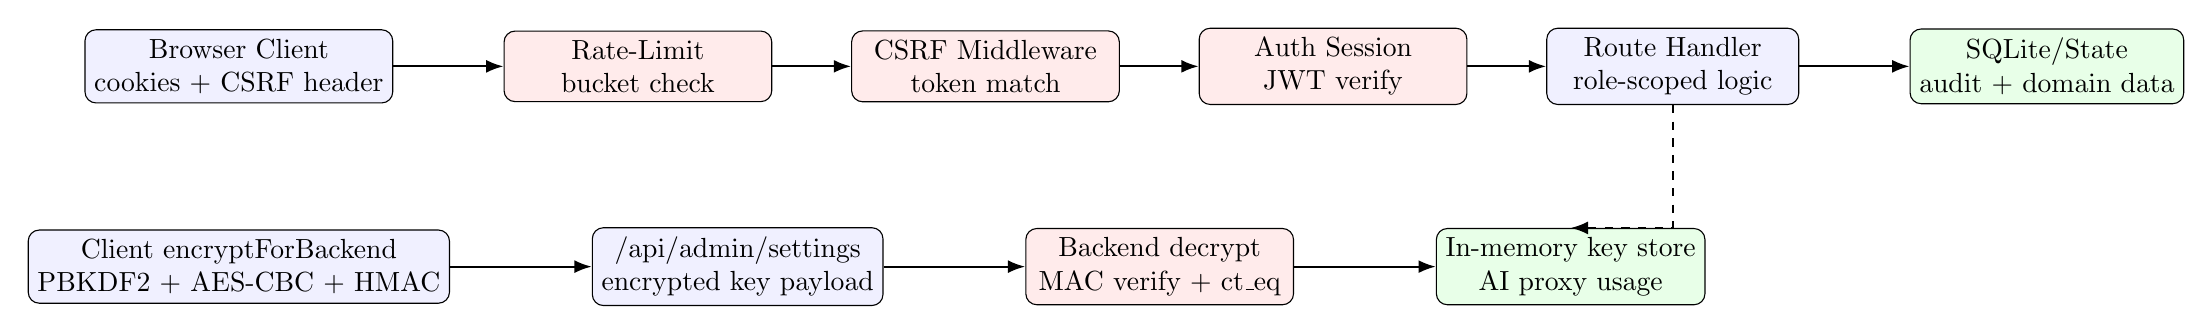
\begin{tikzpicture}[
  node distance=8mm and 10mm,
  box/.style={draw, rounded corners, minimum width=32mm, minimum height=8mm, align=center, fill=blue!6},
  sec/.style={draw, rounded corners, minimum width=34mm, minimum height=8mm, align=center, fill=red!8},
  data/.style={draw, rounded corners, minimum width=34mm, minimum height=8mm, align=center, fill=green!9},
  arrow/.style={-{Latex[length=2.2mm]}, thick}
]
\node[box] (client) {Browser Client\\cookies + CSRF header};
\node[sec, right=14mm of client] (rl) {Rate-Limit\\bucket check};
\node[sec, right=of rl] (csrf) {CSRF Middleware\\token match};
\node[sec, right=of csrf] (auth) {Auth Session\\JWT verify};
\node[box, right=of auth] (handler) {Route Handler\\role-scoped logic};
\node[data, right=14mm of handler] (db) {SQLite/State\\audit + domain data};

\node[box, below=16mm of client] (crypto1) {Client encryptForBackend\\PBKDF2 + AES-CBC + HMAC};
\node[box, right=18mm of crypto1] (crypto2) {/api/admin/settings\\encrypted key payload};
\node[sec, right=18mm of crypto2] (crypto3) {Backend decrypt\\MAC verify + ct\_eq};
\node[data, right=18mm of crypto3] (crypto4) {In-memory key store\\AI proxy usage};

\draw[arrow] (client) -- (rl);
\draw[arrow] (rl) -- (csrf);
\draw[arrow] (csrf) -- (auth);
\draw[arrow] (auth) -- (handler);
\draw[arrow] (handler) -- (db);

\draw[arrow] (crypto1) -- (crypto2);
\draw[arrow] (crypto2) -- (crypto3);
\draw[arrow] (crypto3) -- (crypto4);
\draw[arrow, dashed] (handler.south) |- (crypto4.north);
\end{tikzpicture}
}
\caption{Security-relevant request path and secret-handling path in Open Codelabs.}
\label{fig:security_flow}
\end{figure}

\subsection{Transparent Security Limitations}
The implementation intentionally distinguishes between two client-side encryption contexts:
\begin{itemize}[leftmargin=1.2em]
  \item local browser storage obfuscation (\texttt{encrypt}/\texttt{decrypt}) uses a static client key and should be interpreted as convenience obfuscation rather than strong at-rest protection,
  \item backend-compatible encryption (\texttt{encryptForBackend}) uses password-derived keys and authenticated encryption envelope semantics.
\end{itemize}
In addition, if \texttt{AUTH\_SECRETS} is not set, token signing falls back to \texttt{ADMIN\_PW}; this is explicitly warned in code and should be treated as a deployment hardening requirement \cite{oc_auth_middleware,oc_frontend_crypto}.

\section{Measured Metric Definitions}
\subsection{Scope and Interpretation}
This section defines only metrics that are directly reported in \cref{sec:empirical_eval} or derived from persisted runtime metadata.
No closed-form optimization claim is made from these equations.
The intent is reproducible measurement semantics, not theoretical superiority proof.

\subsection{Completion Metric}
For $N$ attendees and completion indicator $z_i\in\{0,1\}$:
\begin{equation}
C=\frac{1}{N}\sum_{i=1}^{N} z_i.
\label{eq:completion}
\end{equation}
This aligns with requirement-gate enforcement in the runtime model (quiz/feedback/submission toggles).

\subsection{Latency and Token-Cost Decomposition}
For AI request $r$:
\begin{equation}
L_r=L^{net}_{u\rightarrow b}+L^{queue}_{b}+L^{model}_{r}+L^{stream}_{b\rightarrow u}.
\label{eq:latency}
\end{equation}
For $R$ AI requests with token counts $(x_r,y_r)$ and prices $(p_{in},p_{out})$:
\begin{equation}
C_{ai}=\sum_{r=1}^{R}\left(p_{in}x_r+p_{out}y_r\right).
\label{eq:token_cost}
\end{equation}
Because usage metadata is captured directly in stream events, \cref{eq:token_cost} can be estimated from persisted records without replaying traces \cite{oc_gemini_client,oc_ai_handler}.

\subsection{Instantiated Values in This Revision}
Using the internal Basic-vs-Pro ablation artifact (\path{backend/bench-results/reviewer-20260219/ai-ablation.json}), the generation-only totals are:
\begin{itemize}[leftmargin=1.2em]
  \item Basic: 14,507 tokens, 0.0177345 USD,
  \item Pro: 58,000 tokens, 0.0674305 USD.
\end{itemize}
This corresponds to approximately $3.80\times$ higher generation spend for Pro mode in the reported two-task internal sample (\cref{tab:ai_ablation}).
For latency, \cref{eq:latency} is instantiated with measured envelopes from \cref{tab:ws_eval}, where median p95 remained below the 200 ms classroom target up to 100 concurrent users.

\subsection{Localization and Accessibility Reporting Semantics}
Localization and accessibility are reported as concrete inventory/checklist evidence (locale key coverage audits, keyboard/focus/ARIA checks, and theme-mode behavior) rather than a single collapsed score.
This choice avoids over-compressing heterogeneous UI quality signals into one scalar and keeps operator-facing remediation paths explicit.

\section{Verification and Test Evidence}
\subsection{Implemented Automated Tests}
The backend includes integration and module-level tests for critical invariants:
\begin{itemize}[leftmargin=1.2em]
  \item API/session/cookie/CSRF flow and full handler integration \cite{oc_api_tests}.
  \item Public-private visibility and authorization boundaries \cite{oc_visibility_tests}.
  \item Workspace file/git/archive service behavior and failure paths \cite{oc_codeserver_tests}.
  \item Rate-limit window behavior and bucket classification assumptions \cite{oc_rate_limit,oc_security_middleware}.
  \item Audit persistence semantics and failure-tolerant logging behavior \cite{oc_audit_tests}.
\end{itemize}

\begin{table}[t]
\centering
\small
\caption{Test coverage map for high-impact subsystems.}
\label{tab:test_map}
\begin{tabular}{L{0.21\linewidth}L{0.33\linewidth}L{0.36\linewidth}}
\toprule
Subsystem & Covered behaviors & Evidence \\
\midrule
Authentication/session & Login, session cookie flow, CSRF token handling under integration flow & \path{backend/tests/api_tests.rs} \cite{oc_api_tests} \\
Authorization visibility & Private codelab denial for public users, admin-visible supersets & \path{backend/tests/visibility_test.rs} \cite{oc_visibility_tests} \\
Workspace service & Workspace create/write/remove, git init/branch/list/read, archive/remove & \path{backend/src/domain/services/codeserver.rs} \cite{oc_codeserver_tests} \\
Rate limiting & Window rollover and bucket classification logic & \path{backend/src/middleware/rate_limit.rs}, \path{security.rs} \cite{oc_rate_limit,oc_security_middleware} \\
Audit logging & Audit row persistence and non-fatal insertion failure behavior & \path{backend/src/infrastructure/audit.rs} \cite{oc_audit_tests} \\
WebSocket state cleanup & Session cleanup by connection id and attendee-sharing cleanup & \path{backend/src/api/handlers/websocket.rs} \cite{oc_ws_handler} \\
\bottomrule
\end{tabular}
\end{table}

\subsection{Automated Quality Signals from Reproducible SWE Run}
Beyond test presence, we report both the archived SWE artifact (\texttt{backend/bench-results/all-20260219-184314/swe/swe-metrics.json}) and a local refresh run executed for this manuscript update (2026-02-19).
\begin{table}[t]
\centering
\small
\caption{Automated quality metrics from recorded artifact + local refresh run (2026-02-19).}
\label{tab:swe_metrics}
\begin{tabular}{L{0.31\linewidth}L{0.22\linewidth}L{0.37\linewidth}}
\toprule
Check & Result & Notes \\
\midrule
Backend tests (\texttt{cargo test}) & pass (exit 0) & Local refresh run: 31.67 s wall time (167 tests total) \\
Frontend tests (\texttt{bun test --coverage}) & pass (exit 0) & Local refresh run: 52 tests, 8.73 s \\
Backend coverage (\texttt{cargo llvm-cov}, workspace) & lines 74.51\% & Regions 71.28\%, functions 66.77\% \\
Backend coverage (\texttt{cargo llvm-cov}, core service) & lines 95.24\% & Excluding \texttt{src/bin} and \texttt{src/main.rs}: regions 90.54\%, functions 88.13\% \\
Backend lint (\texttt{cargo clippy}) & pass (exit 0) & 54 warnings, 0 errors \\
Frontend static check (\texttt{bun run check}) & pass (exit 0) & Local refresh run: 0 errors, 1 warning (\texttt{EditMode.svelte}) \\
Security audit (\texttt{cargo audit}/\texttt{bun audit}) & findings present & See archived SWE artifact for advisory details and counts \\
\bottomrule
\end{tabular}
\end{table}

\subsection{Representative Test Pseudocode}
\begin{table}[t]
\centering
\small
\caption{Pseudo-code: integration-path test for admin login and codelab roundtrip.}
\label{tab:pseudo_test_integration}
\begin{tabular}{C{0.07\linewidth}L{0.83\linewidth}}
\toprule
Step & Procedure \\
\midrule
1 & Initialize isolated test app state (ephemeral DB + in-memory server context). \\
2 & Execute admin login and collect session cookie + CSRF token. \\
3 & Construct \texttt{CreateCodelab} payload (title, description, author, default requirement flags). \\
4 & Call \texttt{POST /api/codelabs} with auth headers and payload; assert HTTP 201. \\
5 & Parse created codelab identifier from response body. \\
6 & Call \texttt{GET /api/codelabs/\{id\}} with same auth context; assert HTTP 200. \\
7 & Verify persisted fields match request payload (\texttt{title}, \texttt{author}, visibility defaults). \\
\bottomrule
\end{tabular}
\end{table}

\begin{table}[t]
\centering
\small
\caption{Pseudo-code: workspace service test for branch creation and file listing invariants.}
\label{tab:pseudo_test_workspace}
\begin{tabular}{C{0.07\linewidth}L{0.83\linewidth}}
\toprule
Step & Procedure \\
\midrule
1 & Create temporary workspace root and instantiate \texttt{CodeServerManager}. \\
2 & Create workspace named \texttt{branch-test}. \\
3 & Initialize git repository for \texttt{branch-test}. \\
4 & Write \texttt{README.md} with seed content and commit initial changes. \\
5 & Create step branch (\texttt{step=1}, name=\texttt{start}). \\
6 & List workspace branches and assert the branch set contains \texttt{start}. \\
7 & List files on branch \texttt{start} and assert \texttt{README.md} is present. \\
\bottomrule
\end{tabular}
\end{table}

\subsection{Role-Oriented Verification Matrix}
Beyond isolated module tests, workshop reliability depends on multi-role behavioral consistency.
\cref{tab:role_verification} maps high-impact facilitator/attendee behaviors to concrete failure classes that should be validated before release deployments.

\begin{table}[t]
\centering
\small
\caption{Role-oriented verification matrix for release readiness.}
\label{tab:role_verification}
\begin{tabular}{L{0.22\linewidth}L{0.30\linewidth}L{0.34\linewidth}}
\toprule
Role flow & Failure class & Verification focus \\
\midrule
Facilitator login and settings & Session/CSRF mismatch & Cookie issuance, CSRF header requirement, secure logout semantics \\
Attendee registration and progression & Identity collision / scope leak & Duplicate-name handling, codelab-bound attendee token constraints \\
Live help triage and DM & Misrouted messaging & Correct target fan-out to multi-tab sessions, state transition pending$\rightarrow$resolved \\
AI assistant usage & Policy bypass / noisy failures & Model allow-list, prompt validation, graceful surfacing of rate/timeout errors \\
Workspace snapshot operations & Data loss or corruption & Branch/folder file integrity, archive completeness, deletion guard behavior \\
Completion and certificate path & Incorrect eligibility & Requirement-gate toggles and derived completion consistency \\
\bottomrule
\end{tabular}
\end{table}

\section{Empirical Evaluation}
\label{sec:empirical_eval}
\subsection{Evaluation Questions}
This revision addresses reviewer-raised evidence gaps with four explicit questions:
\begin{itemize}[leftmargin=1.2em]
  \item \textbf{EQ1:} What latency/error envelope is observed on core REST control paths?
  \item \textbf{EQ2:} How does WebSocket roundtrip latency scale with concurrent attendees?
  \item \textbf{EQ3:} Does Pro-mode staged generation improve quality proxies over Basic mode, and at what token/cost overhead?
  \item \textbf{EQ4:} Is the system operationally stable in deployment-style rehearsal runs?
\end{itemize}

\subsection{Measurement Setup and Reproducibility}
\begin{table}[t]
\centering
\small
\caption{Evaluation environment and artifact locations for this manuscript revision.}
\label{tab:eval_setup}
\begin{tabular}{L{0.30\linewidth}L{0.62\linewidth}}
\toprule
Item & Value \\
\midrule
Repository snapshot & \texttt{a3510b39} \\
Host platform & macOS 15.7.4 (arm64), 10 CPU cores, 16 GB RAM \\
Backend runtime & Rust release build (\texttt{cargo run --release --bin backend}) \\
Frontend runtime (route benchmark) & SvelteKit/Bun on \texttt{http://localhost:5173} \\
Benchmark harness & \texttt{backend/bench/run\_all\_local.sh}, \texttt{run\_matrix.sh}, \texttt{ai\_mode\_ablation.py} \\
Primary result artifacts & \texttt{backend/bench-results/reviewer-20260219/*} and \texttt{backend/bench-results/all-20260219-184314/*} \\
Rate-limit policy during load tests & high benchmark envelope (\texttt{RATE\_LIMIT\_\{GENERAL,LOGIN,AI,UPLOAD\}*=10000}) \\
\bottomrule
\end{tabular}
\end{table}
For stability against run-to-run variance, EQ1 REST control paths were repeated 5 times per attendee cardinality (\texttt{local-a10-r1..r5}, \texttt{local-a50-r1..r5}) and EQ2 WebSocket runs were repeated 3 times per concurrency point (\texttt{ws-u\{5,20,50,100\}-r1..r3}).

\subsection{REST Control-Path Latency (EQ1)}
\begin{table}[H]
\centering
\small
\caption{REST p95 latency summaries under two attendee cardinalities (median [Q1,Q3], 5 repeats each).}
\label{tab:rest_eval}
\begin{tabular}{L{0.36\linewidth}C{0.24\linewidth}C{0.24\linewidth}}
\toprule
Scenario & p95 @10 attendees (ms) & p95 @50 attendees (ms) \\
\midrule
\texttt{admin\_get\_attendees} & 1420.4 [875.1, 1423.2] & 7228.8 [4365.0, 8419.0] \\
\texttt{admin\_get\_chat\_history} & 6.1 [3.5, 8.3] & 7.9 [6.5, 11.3] \\
\texttt{attendee\_post\_help} & 23.6 [23.2, 37.7] & 24.2 [23.7, 24.3] \\
\texttt{attendee\_post\_submission\_link} & 21.8 [12.6, 37.8] & 24.6 [22.6, 24.6] \\
\bottomrule
\end{tabular}
\end{table}
All 10 repeated runs (5 at each attendee setting) stayed error-free on these control paths, but \texttt{admin\_get\_attendees} is a clear latency hotspot and dominates p95 under larger attendee sets.
This quantitatively identifies where indexing/query-shape optimization should be prioritized before larger live events.

\subsection{WebSocket Scaling (EQ2)}
\begin{table}[H]
\centering
\small
\caption{WebSocket chat roundtrip summaries across concurrency levels (median [Q1,Q3], 3 repeats each).}
\label{tab:ws_eval}
\begin{tabular}{C{0.10\linewidth}C{0.19\linewidth}C{0.19\linewidth}C{0.19\linewidth}C{0.23\linewidth}}
\toprule
Users & p50 (ms) & p95 (ms) & p99 (ms) & Delivery ratio \\
\midrule
5 & 11.9 [11.2, 16.7] & 42.2 [34.5, 66.8] & 42.9 [39.0, 71.9] & 1.000 [1.000, 1.000] \\
20 & 13.4 [12.8, 15.6] & 65.7 [54.0, 113.0] & 96.7 [82.0, 143.6] & 1.000 [0.999, 1.000] \\
50 & 23.0 [21.2, 23.9] & 47.8 [45.5, 54.9] & 67.1 [66.5, 79.5] & 0.995 [0.992, 0.996] \\
100 & 45.1 [44.5, 45.8] & 99.3 [94.0, 108.9] & 119.8 [109.3, 126.5] & 0.999 [0.998, 0.999] \\
\bottomrule
\end{tabular}
\end{table}
The 100-user case remained below the 200 ms p95 classroom target across repeats (median 99.29 ms, IQR 94.00--108.94 ms).
Harness-level disconnect/error counters include teardown resets; delivery ratio remained high (median $\ge 0.995$ at all tested loads).

\begin{figure}[H]
\centering
\resizebox{0.90\linewidth}{!}{
\begin{tikzpicture}[x=1.1cm,y=0.035cm]
  \draw[->, thick] (0,0) -- (8.4,0) node[right] {Concurrent users};
  \draw[->, thick] (0,0) -- (0,230) node[above] {WebSocket p95 (ms)};
  \draw[dashed] (0,200) -- (10,200) node[right] {Target 200 ms};

  \foreach \x/\label in {1/5,3/20,5/50,7/100}
    \draw (\x,0) -- (\x,-6) node[below] {\label};
  \foreach \y in {0,50,100,150,200}
    \draw (0,\y) -- (-0.2,\y) node[left] {\y};

  \draw[blue, thick] (1,42.22) -- (3,65.66) -- (5,47.78) -- (7,99.29);
  \foreach \x/\y/\qone/\qthree in {
    1/42.22/34.46/66.84,
    3/65.66/54.04/112.98,
    5/47.78/45.54/54.86,
    7/99.29/94.00/108.94}
  {
    \draw[blue] (\x,\qone) -- (\x,\qthree);
    \filldraw[blue] (\x,\y) circle (2pt);
  }
\end{tikzpicture}
}
\caption{Observed WebSocket p95 latency scaling from 5 to 100 concurrent users (point: median, bar: IQR, 3 repeats each).}
\label{fig:ws_p95_scaling}
\end{figure}

\subsection{Operational I/O and Frontend Route Results (EQ1, EQ4)}
\begin{table}[t]
\centering
\scriptsize
\caption{Representative operational-path benchmark results.}
\label{tab:ops_eval}
\begin{tabular}{L{0.25\linewidth}L{0.13\linewidth}L{0.50\linewidth}}
\toprule
Scenario class & Metric & Observed value \\
\midrule
Upload (1 MB, concurrency 4) & p95 latency & 11.13 ms, 12/12 success \\
Upload (3 MB, concurrency 4) & p95 latency & 33.31 ms, 12/12 success \\
Backup tiny dataset & export / inspect / restore & 75.93 / 59.95 / 254.46 ms; all status 200 \\
Backup small dataset & export / inspect / restore & 61.75 / 90.79 / 213.79 ms; all status 200 \\
Code-server workspace & create / download & 54.81 / 30.67 ms \\
Code-server updates & branch p95 / folder p95 & 75.25 / 0.94 ms \\
Frontend route (\texttt{/}, c=4) & p95 latency & 104.09 ms, 0.0\% error \\
Frontend route (\texttt{/admin}, c=4) & p95 latency & 105.10 ms, 0.0\% error \\
\bottomrule
\end{tabular}
\end{table}

\subsection{AI Quality-Cost Ablation: Basic vs Pro (EQ3)}
We ran an internal pilot ablation on two backend tasks (\texttt{ai.rs}, \texttt{websocket.rs}) using the same model family (\texttt{gemini-3-flash-preview}), comparing:
\begin{itemize}[leftmargin=1.2em]
  \item \textbf{Basic mode}: single-pass structured generation.
  \item \textbf{Pro mode}: Plan $\rightarrow$ Draft $\rightarrow$ Review $\rightarrow$ Revise.
\end{itemize}
Both outputs were audited using the same review schema to compute comparable issue/missing-item counts.
This is explicitly a directional engineering signal ($n=2$), not a statistically powered quality study.

\begin{table}[t]
\centering
\small
\caption{Basic vs Pro ablation summary (internal pilot, $n=2$ tasks).}
\label{tab:ai_ablation}
\begin{tabular}{L{0.34\linewidth}C{0.21\linewidth}C{0.21\linewidth}}
\toprule
Metric & Basic & Pro \\
\midrule
Mean issues per task & 5.5 & 4.5 \\
Mean missing items per task & 5.5 & 4.0 \\
Mean section-hits score & 3.0 & 4.0 \\
Total generation tokens & 14,507 & 58,000 \\
Total generation cost (USD) & 0.0177345 & 0.0674305 \\
Cost per task (USD) & 0.0088673 & 0.0337153 \\
\bottomrule
\end{tabular}
\end{table}
Relative to Basic mode, Pro mode reduced mean issue count by 18.18\% and missing-item count by 27.27\%, while increasing token/cost load by about $4\times$.
With only two tasks, we do not report inferential statistics or generalization claims; this quantifies a local governance trade-off under one internal workload.

\subsection{Deployment-Style Pilot Evidence (EQ4)}
For operational validation beyond microbenchmarks, we include two deployment-oriented signals:
\begin{itemize}[leftmargin=1.2em]
  \item soak rehearsal artifact (\texttt{backend/bench-results/all-20260219-184314/soak/soak.json}): 1/1 successful cycle, no failed cycles;
  \item project FAQ field report: stable operation at 100 concurrent users and tested up to 200 users with rising CPU pressure \cite{oc_faq_en_doc}.
\end{itemize}
This is not yet a randomized educational-outcome study, but it provides concrete operations evidence from both instrumented rehearsal and prior deployment practice.

\subsection{Evidence Gaps and Next-Phase Evaluation Protocol}
To address reviewer concerns on scientific rigor, the next revision is scoped with explicit minimum evidence targets:
\begin{enumerate}[leftmargin=1.2em]
  \item \textbf{Human workshop study:} at least one controlled facilitator-attendee deployment comparing Open Codelabs with a multi-tool baseline, with measured intervention latency and post-session learner/facilitator feedback.
  \item \textbf{Scaled AI benchmark:} 50--100 codelab-generation tasks with blinded human rating on pedagogy, correctness, and structural completeness (Basic vs Pro vs external one-pass baseline).
  \item \textbf{Agent-stage ablation:} isolate stage impact (e.g., Basic, Basic+Review, Plan+Draft, full Pro) to identify which stage contributes measurable gains.
  \item \textbf{Independent review channel:} separate evaluator model and human raters from generator model family to reduce same-model bias.
\end{enumerate}
The current manuscript includes only the operational pilot evidence; the protocol above defines the acceptance-bar expansion path rather than claiming it is already complete.

\section{Limitations, Risks, and Future Work}
Current constraints include single-node real-time fan-out assumptions, facilitator-centric trust model for sensitive operations, and dependence on external model behavior for AI output quality.
From an evaluation perspective, this revision still has important limits:
\begin{itemize}[leftmargin=1.2em]
  \item the AI ablation sample is small ($n=2$ tasks) and uses one model family for both generation and schema-based review;
  \item no external codelab-generator baseline (outside this codebase) is included in the current EQ3 run;
  \item deployment evidence is rehearsal/field-report oriented, not a randomized controlled educational-outcome trial;
  \item WebSocket disconnect/error counters in the harness include teardown resets and should not be interpreted as production outage rate.
\end{itemize}
Even with structured output and staged prompting, generative errors remain possible, especially when source context is incomplete or ambiguous.

Future work priorities:
\begin{enumerate}[leftmargin=1.2em]
  \item Distributed WebSocket architecture with shared message broker for larger cohorts.
  \item Controlled workshop studies with human raters and blinded Basic-vs-Pro scoring for pedagogical quality.
  \item Longitudinal learning-outcome analysis beyond session-completion proxies.
  \item Adaptive support scheduling with empirically calibrated request-priority features from real classroom traces.
  \item Formal prompt/version governance with regression tests over representative codelab corpora and explicit token-budget guardrails.
\end{enumerate}

\section{Conclusion}
Open Codelabs demonstrates that a modern workshop platform can unify facilitator operations, attendee learning flow, governance controls, and AI-assisted content lifecycle in one architecture.
The implementation goes beyond static codelab rendering: it includes live classroom control, structured AI pipelines, optional workspaces, multilingual runtime support, and accessibility-aware UI behavior.
This revised report adds empirical evidence for latency scaling, operational-path performance, and Basic-vs-Pro AI quality/cost trade-offs, while explicitly reporting current evaluation limits.
It documents capabilities at code-level granularity and provides transparent artifacts for reproducibility, including explicit route maps and prompt templates.

\begin{thebibliography}{10}

\bibitem{bun}
{Bun Contributors}.
\newblock Bun runtime.
\newblock \url{https://bun.sh/}, 2026.
\newblock Accessed: 2026-02-18.

\bibitem{rw_cloudcoder}
{CloudCoder Contributors}.
\newblock Cloudcoder: A web-based programming exercise and assessment system.
\newblock \url{https://github.com/cloudcoderdotorg/CloudCoder}, 2026.
\newblock Accessed: 2026-02-18.

\bibitem{rw_code_server_docs}
{Coder Technologies, Inc.}
\newblock code-server documentation.
\newblock \url{https://coder.com/docs/code-server}, 2026.
\newblock Accessed: 2026-02-18.

\bibitem{rw_github_classroom}
{GitHub}.
\newblock Github classroom.
\newblock \url{https://classroom.github.com/}, 2026.
\newblock Accessed: 2026-02-18.

\bibitem{rw_google_codelabs_tools}
{Google Codelabs Contributors}.
\newblock Google codelabs tools.
\newblock \url{https://github.com/googlecodelabs/tools}, 2026.
\newblock Accessed: 2026-02-18.

\bibitem{rw_sqkt}
Doyoun Kim, Suin Kim, and Yojan Jo.
\newblock Knowledge tracing in programming education integrating students'
  questions.
\newblock {\em arXiv preprint arXiv:2502.10408}, 2025.

\bibitem{sqlx}
{Launchbadge Contributors}.
\newblock Sqlx.
\newblock \url{https://github.com/launchbadge/sqlx}, 2026.
\newblock Accessed: 2026-02-18.

\bibitem{rw_coderunner_agent}
Huiyong Li and Boxuan Ma.
\newblock Design of ai-powered tool for self-regulation support in programming
  education.
\newblock {\em arXiv preprint arXiv:2504.03068}, 2025.

\bibitem{rw_chatgpt_case_study}
Boxaun Ma, Li~Chen, and Shin'ichi Konomi.
\newblock Enhancing programming education with chatgpt: A case study on student
  perceptions and interactions in a python course.
\newblock {\em arXiv preprint arXiv:2403.15472}, 2024.

\bibitem{rw_auto_grading_review}
Marcus Messer, Neil C.~C. Brown, Michael K{\"o}lling, and Miaojing Shi.
\newblock Automated grading and feedback tools for programming education: A
  systematic review.
\newblock {\em arXiv preprint arXiv:2306.11722}, 2023.

\bibitem{oc_admin_handler}
{Open Codelabs Contributors}.
\newblock Open codelabs admin handler.
\newblock
  \url{https://github.com/JAICHANGPARK/open-codelabs/blob/main/backend/src/api/handlers/admin.rs},
  2026.
\newblock Accessed: 2026-02-18.

\bibitem{oc_ai_generator_component}
{Open Codelabs Contributors}.
\newblock Open codelabs ai codelab generator component.
\newblock
  \url{https://github.com/JAICHANGPARK/open-codelabs/blob/main/frontend/src/lib/components/admin/AiCodelabGenerator.svelte},
  2026.
\newblock Accessed: 2026-02-18.

\bibitem{oc_ai_handler}
{Open Codelabs Contributors}.
\newblock Open codelabs ai handler (proxy, conversations, threads).
\newblock
  \url{https://github.com/JAICHANGPARK/open-codelabs/blob/main/backend/src/api/handlers/ai.rs},
  2026.
\newblock Accessed: 2026-02-18.

\bibitem{oc_api_reference_doc}
{Open Codelabs Contributors}.
\newblock Open codelabs api reference.
\newblock
  \url{https://github.com/JAICHANGPARK/open-codelabs/blob/main/docs/en/specification/api-reference.md},
  2026.
\newblock Accessed: 2026-02-18.

\bibitem{oc_routes}
{Open Codelabs Contributors}.
\newblock Open codelabs api route definitions.
\newblock
  \url{https://github.com/JAICHANGPARK/open-codelabs/blob/main/backend/src/api/routes.rs},
  2026.
\newblock Accessed: 2026-02-18.

\bibitem{oc_ask_gemini_component}
{Open Codelabs Contributors}.
\newblock Open codelabs ask gemini component.
\newblock
  \url{https://github.com/JAICHANGPARK/open-codelabs/blob/main/frontend/src/lib/components/codelabs/AskGemini.svelte},
  2026.
\newblock Accessed: 2026-02-18.

\bibitem{oc_attendees_handler}
{Open Codelabs Contributors}.
\newblock Open codelabs attendee handler.
\newblock
  \url{https://github.com/JAICHANGPARK/open-codelabs/blob/main/backend/src/api/handlers/attendees.rs},
  2026.
\newblock Accessed: 2026-02-18.

\bibitem{oc_audit_tests}
{Open Codelabs Contributors}.
\newblock Open codelabs audit logging infrastructure and tests.
\newblock
  \url{https://github.com/JAICHANGPARK/open-codelabs/blob/main/backend/src/infrastructure/audit.rs},
  2026.
\newblock Accessed: 2026-02-18.

\bibitem{oc_auth_middleware}
{Open Codelabs Contributors}.
\newblock Open codelabs authentication middleware.
\newblock
  \url{https://github.com/JAICHANGPARK/open-codelabs/blob/main/backend/src/middleware/auth.rs},
  2026.
\newblock Accessed: 2026-02-18.

\bibitem{oc_api_tests}
{Open Codelabs Contributors}.
\newblock Open codelabs backend api integration tests.
\newblock
  \url{https://github.com/JAICHANGPARK/open-codelabs/blob/main/backend/tests/api_tests.rs},
  2026.
\newblock Accessed: 2026-02-18.

\bibitem{oc_arch_backend_doc}
{Open Codelabs Contributors}.
\newblock Open codelabs backend architecture document.
\newblock
  \url{https://github.com/JAICHANGPARK/open-codelabs/blob/main/docs/en/architecture/backend.md},
  2026.
\newblock Accessed: 2026-02-18.

\bibitem{oc_backend_cargo_toml}
{Open Codelabs Contributors}.
\newblock Open codelabs backend cargo manifest.
\newblock
  \url{https://github.com/JAICHANGPARK/open-codelabs/blob/main/backend/Cargo.toml},
  2026.
\newblock Accessed: 2026-02-18.

\bibitem{oc_backend_crypto}
{Open Codelabs Contributors}.
\newblock Open codelabs backend cryptography utility.
\newblock
  \url{https://github.com/JAICHANGPARK/open-codelabs/blob/main/backend/src/utils/crypto.rs},
  2026.
\newblock Accessed: 2026-02-18.

\bibitem{oc_backend_dockerfile}
{Open Codelabs Contributors}.
\newblock Open codelabs backend dockerfile.
\newblock
  \url{https://github.com/JAICHANGPARK/open-codelabs/blob/main/backend/Dockerfile},
  2026.
\newblock Accessed: 2026-02-18.

\bibitem{oc_main_rs}
{Open Codelabs Contributors}.
\newblock Open codelabs backend entrypoint (main.rs).
\newblock
  \url{https://github.com/JAICHANGPARK/open-codelabs/blob/main/backend/src/main.rs},
  2026.
\newblock Accessed: 2026-02-18.

\bibitem{oc_codeserver_tests}
{Open Codelabs Contributors}.
\newblock Open codelabs codeserver service and tests.
\newblock
  \url{https://github.com/JAICHANGPARK/open-codelabs/blob/main/backend/src/domain/services/codeserver.rs},
  2026.
\newblock Accessed: 2026-02-18.

\bibitem{oc_db_schema_doc}
{Open Codelabs Contributors}.
\newblock Open codelabs database schema document.
\newblock
  \url{https://github.com/JAICHANGPARK/open-codelabs/blob/main/docs/en/specification/database-schema.md},
  2026.
\newblock Accessed: 2026-02-18.

\bibitem{oc_docker_compose}
{Open Codelabs Contributors}.
\newblock Open codelabs docker compose configuration.
\newblock
  \url{https://github.com/JAICHANGPARK/open-codelabs/blob/main/docker-compose.yml},
  2026.
\newblock Accessed: 2026-02-18.

\bibitem{oc_env_sample}
{Open Codelabs Contributors}.
\newblock Open codelabs environment variable sample.
\newblock
  \url{https://github.com/JAICHANGPARK/open-codelabs/blob/main/.env.sample},
  2026.
\newblock Accessed: 2026-02-18.

\bibitem{oc_consultant_component}
{Open Codelabs Contributors}.
\newblock Open codelabs facilitator consultant component.
\newblock
  \url{https://github.com/JAICHANGPARK/open-codelabs/blob/main/frontend/src/lib/components/admin/FacilitatorConsultant.svelte},
  2026.
\newblock Accessed: 2026-02-18.

\bibitem{oc_faq_en_doc}
{Open Codelabs Contributors}.
\newblock Open codelabs faq (english).
\newblock
  \url{https://github.com/JAICHANGPARK/open-codelabs/blob/main/docs/en/faq.md},
  2026.
\newblock Accessed: 2026-02-19.

\bibitem{open_codelabs_features_doc}
{Open Codelabs Contributors}.
\newblock Open codelabs feature specification.
\newblock
  \url{https://github.com/JAICHANGPARK/open-codelabs/blob/main/docs/en/specification/features.md},
  2026.
\newblock Accessed: 2026-02-18.

\bibitem{oc_focus_trap}
{Open Codelabs Contributors}.
\newblock Open codelabs focus trap component.
\newblock
  \url{https://github.com/JAICHANGPARK/open-codelabs/blob/main/frontend/src/lib/components/FocusTrap.svelte},
  2026.
\newblock Accessed: 2026-02-18.

\bibitem{oc_frontend_api_selector}
{Open Codelabs Contributors}.
\newblock Open codelabs frontend api mode selector.
\newblock
  \url{https://github.com/JAICHANGPARK/open-codelabs/blob/main/frontend/src/lib/api.ts},
  2026.
\newblock Accessed: 2026-02-18.

\bibitem{oc_arch_frontend_doc}
{Open Codelabs Contributors}.
\newblock Open codelabs frontend architecture document.
\newblock
  \url{https://github.com/JAICHANGPARK/open-codelabs/blob/main/docs/en/architecture/frontend.md},
  2026.
\newblock Accessed: 2026-02-18.

\bibitem{oc_api_backend_client}
{Open Codelabs Contributors}.
\newblock Open codelabs frontend backend api client.
\newblock
  \url{https://github.com/JAICHANGPARK/open-codelabs/blob/main/frontend/src/lib/api-backend.ts},
  2026.
\newblock Accessed: 2026-02-18.

\bibitem{oc_frontend_dockerfile}
{Open Codelabs Contributors}.
\newblock Open codelabs frontend dockerfile.
\newblock
  \url{https://github.com/JAICHANGPARK/open-codelabs/blob/main/frontend/Dockerfile},
  2026.
\newblock Accessed: 2026-02-18.

\bibitem{oc_frontend_crypto}
{Open Codelabs Contributors}.
\newblock Open codelabs frontend encryption helper.
\newblock
  \url{https://github.com/JAICHANGPARK/open-codelabs/blob/main/frontend/src/lib/crypto.ts},
  2026.
\newblock Accessed: 2026-02-18.

\bibitem{oc_frontend_package_json}
{Open Codelabs Contributors}.
\newblock Open codelabs frontend package manifest.
\newblock
  \url{https://github.com/JAICHANGPARK/open-codelabs/blob/main/frontend/package.json},
  2026.
\newblock Accessed: 2026-02-18.

\bibitem{oc_frontend_hooks}
{Open Codelabs Contributors}.
\newblock Open codelabs frontend server hooks security header logic.
\newblock
  \url{https://github.com/JAICHANGPARK/open-codelabs/blob/main/frontend/src/hooks.server.ts},
  2026.
\newblock Accessed: 2026-02-18.

\bibitem{oc_gemini_client}
{Open Codelabs Contributors}.
\newblock Open codelabs gemini client utilities.
\newblock
  \url{https://github.com/JAICHANGPARK/open-codelabs/blob/main/frontend/src/lib/gemini.ts},
  2026.
\newblock Accessed: 2026-02-18.

\bibitem{oc_app_css}
{Open Codelabs Contributors}.
\newblock Open codelabs global styles (theme and accessibility variables).
\newblock
  \url{https://github.com/JAICHANGPARK/open-codelabs/blob/main/frontend/src/app.css},
  2026.
\newblock Accessed: 2026-02-18.

\bibitem{oc_guide_pipeline_component}
{Open Codelabs Contributors}.
\newblock Open codelabs guide generation pipeline (admin page).
\newblock
  \url{https://github.com/JAICHANGPARK/open-codelabs/blob/main/frontend/src/routes/admin/[id]/+page.svelte},
  2026.
\newblock Accessed: 2026-02-18.

\bibitem{oc_i18n_index}
{Open Codelabs Contributors}.
\newblock Open codelabs i18n locale registry.
\newblock
  \url{https://github.com/JAICHANGPARK/open-codelabs/blob/main/frontend/src/lib/i18n/index.ts},
  2026.
\newblock Accessed: 2026-02-18.

\bibitem{oc_installation_en_doc}
{Open Codelabs Contributors}.
\newblock Open codelabs installation guide (english).
\newblock
  \url{https://github.com/JAICHANGPARK/open-codelabs/blob/main/docs/en/getting-started/installation.md},
  2026.
\newblock Accessed: 2026-02-19.

\bibitem{oc_landing_page}
{Open Codelabs Contributors}.
\newblock Open codelabs landing page (pro workflow and agent graph).
\newblock
  \url{https://github.com/JAICHANGPARK/open-codelabs/blob/main/landing/src/routes/+page.svelte},
  2026.
\newblock Accessed: 2026-02-18.

\bibitem{open_codelabs_overview_doc}
{Open Codelabs Contributors}.
\newblock Open codelabs project overview.
\newblock
  \url{https://github.com/JAICHANGPARK/open-codelabs/blob/main/docs/specification/overview.md},
  2026.
\newblock Accessed: 2026-02-18.

\bibitem{oc_rate_limit}
{Open Codelabs Contributors}.
\newblock Open codelabs rate limiting middleware.
\newblock
  \url{https://github.com/JAICHANGPARK/open-codelabs/blob/main/backend/src/middleware/rate_limit.rs},
  2026.
\newblock Accessed: 2026-02-18.

\bibitem{open_codelabs_readme}
{Open Codelabs Contributors}.
\newblock Open codelabs readme.
\newblock
  \url{https://github.com/JAICHANGPARK/open-codelabs/blob/main/README.md},
  2026.
\newblock Accessed: 2026-02-18.

\bibitem{oc_layout}
{Open Codelabs Contributors}.
\newblock Open codelabs root layout (locale, theme, accessibility controls).
\newblock
  \url{https://github.com/JAICHANGPARK/open-codelabs/blob/main/frontend/src/routes/+layout.svelte},
  2026.
\newblock Accessed: 2026-02-18.

\bibitem{oc_security_middleware}
{Open Codelabs Contributors}.
\newblock Open codelabs security middleware (headers, csrf, rate limit).
\newblock
  \url{https://github.com/JAICHANGPARK/open-codelabs/blob/main/backend/src/middleware/security.rs},
  2026.
\newblock Accessed: 2026-02-18.

\bibitem{oc_db_dml_queries}
{Open Codelabs Contributors}.
\newblock Open codelabs sql dml in api handlers and audit infrastructure.
\newblock
  \url{https://github.com/JAICHANGPARK/open-codelabs/tree/main/backend/src/api/handlers},
  2026.
\newblock Accessed: 2026-02-18.

\bibitem{oc_migrations_dir}
{Open Codelabs Contributors}.
\newblock Open codelabs sql migration corpus.
\newblock
  \url{https://github.com/JAICHANGPARK/open-codelabs/tree/main/backend/migrations},
  2026.
\newblock Accessed: 2026-02-18.

\bibitem{oc_arch_system_doc}
{Open Codelabs Contributors}.
\newblock Open codelabs system architecture document.
\newblock
  \url{https://github.com/JAICHANGPARK/open-codelabs/blob/main/docs/en/architecture/system-architecture.md},
  2026.
\newblock Accessed: 2026-02-18.

\bibitem{oc_theme_state}
{Open Codelabs Contributors}.
\newblock Open codelabs theme state manager.
\newblock
  \url{https://github.com/JAICHANGPARK/open-codelabs/blob/main/frontend/src/lib/theme.svelte.ts},
  2026.
\newblock Accessed: 2026-02-18.

\bibitem{oc_check_i18n_script}
{Open Codelabs Contributors}.
\newblock Open codelabs translation audit script.
\newblock
  \url{https://github.com/JAICHANGPARK/open-codelabs/blob/main/frontend/scripts/check-i18n.mjs},
  2026.
\newblock Accessed: 2026-02-18.

\bibitem{oc_visibility_tests}
{Open Codelabs Contributors}.
\newblock Open codelabs visibility and authorization tests.
\newblock
  \url{https://github.com/JAICHANGPARK/open-codelabs/blob/main/backend/tests/visibility_test.rs},
  2026.
\newblock Accessed: 2026-02-18.

\bibitem{oc_ws_handler}
{Open Codelabs Contributors}.
\newblock Open codelabs websocket handler.
\newblock
  \url{https://github.com/JAICHANGPARK/open-codelabs/blob/main/backend/src/api/handlers/websocket.rs},
  2026.
\newblock Accessed: 2026-02-18.

\bibitem{rw_gitseed}
Pedro Orvalho, Mikolas Janota, and Vasco Manquinho.
\newblock Gitseed: A git-backed automated assessment tool for software
  engineering and programming education.
\newblock {\em arXiv preprint arXiv:2409.07362}, 2024.

\bibitem{rw_genai_benchmark}
Tung Phung, Victor-Alexandru Padurean, Jose Cambronero, Sumit Gulwani, Tobias
  Kohn, Rupak Majumdar, Adish Singla, and Gustavo Soares.
\newblock Generative ai for programming education: Benchmarking chatgpt, gpt-4,
  and human tutors.
\newblock {\em arXiv preprint arXiv:2306.17156}, 2023.

\bibitem{rw_llm_apps_survey}
Griffin Pitts, Anurata~Prabha Hridi, and Arun-Balajiee Lekshmi-Narayanan.
\newblock A survey of llm-based applications in programming education:
  Balancing automation and human oversight.
\newblock {\em arXiv preprint arXiv:2510.03719}, 2025.

\bibitem{rw_pedagogical_sft}
Emily Ross, Yuval Kansal, Jake Renzella, Alexandra Vassar, and Andrew Taylor.
\newblock Supervised fine-tuning llms to behave as pedagogical agents in
  programming education.
\newblock {\em arXiv preprint arXiv:2502.20527}, 2025.

\bibitem{rw_classcode}
Ryo Suzuki, Jun Kato, and Koji Yatani.
\newblock Classcode: An interactive teaching and learning environment for
  programming education in classrooms.
\newblock {\em arXiv preprint arXiv:2001.08194}, 2020.

\bibitem{sveltekit}
{Svelte Team}.
\newblock Sveltekit documentation.
\newblock \url{https://svelte.dev/docs/kit}, 2026.
\newblock Accessed: 2026-02-18.

\bibitem{axum}
{Tokio Contributors}.
\newblock Axum web framework.
\newblock \url{https://github.com/tokio-rs/axum}, 2026.
\newblock Accessed: 2026-02-18.

\bibitem{tokio}
{Tokio Contributors}.
\newblock Tokio asynchronous runtime.
\newblock \url{https://tokio.rs/}, 2026.
\newblock Accessed: 2026-02-18.

\bibitem{rw_marmoset}
{University of Maryland}.
\newblock Marmoset project.
\newblock \url{https://marmoset.cs.umd.edu/}, 2026.
\newblock Accessed: 2026-02-18.

\bibitem{rw_llm_prog_review}
Meina Zhu, Lanyu Xu, and Barbara Ericson.
\newblock A systematic review of research on large language models for computer
  programming education.
\newblock {\em arXiv preprint arXiv:2506.21818}, 2025.

\end{thebibliography}


\appendix

\section{Complete API Route Catalog}
\label{app:api}
\small
\begin{longtable}{L{0.07\linewidth}T{0.40\linewidth}L{0.14\linewidth}L{0.25\linewidth}}
\caption{Route-level API surface (from backend router).}
\label{tab:api_catalog}\\
\toprule
Method & Path & Typical access & Purpose \\
\midrule
\endfirsthead
\toprule
Method & Path & Typical access & Purpose \\
\midrule
\endhead
\midrule
\multicolumn{4}{r}{Continued on next page} \\
\midrule
\endfoot
\bottomrule
\endlastfoot
POST & \path{/api/login} & Public & Admin login session creation \\
POST & \path{/api/logout} & Session user & Session termination \\
GET & \path{/api/session} & Session user & Session role introspection \\

POST & \path{/api/admin/settings} & Admin & Update admin-level settings \\
GET & \path{/api/admin/updates} & Admin & Version/update check \\
GET & \path{/api/admin/audit-logs} & Admin & Audit log retrieval \\
GET & \path{/api/admin/backup/export} & Admin & Backup export \\
POST & \path{/api/admin/backup/inspect} & Admin & Backup inspection \\
POST & \path{/api/admin/backup/restore} & Admin & Backup restore \\

GET & \path{/api/codelabs/reference} & Public/Admin & Reference codelab list \\
GET & \path{/api/codelabs} & Public/Admin & List codelabs (visibility-aware) \\
POST & \path{/api/codelabs} & Admin & Create codelab \\
GET & \path{/api/codelabs/:id} & Public/Admin & Get one codelab \\
PUT & \path{/api/codelabs/:id} & Admin & Update codelab metadata \\
DELETE & \path{/api/codelabs/:id} & Admin & Delete codelab \\
POST & \path{/api/codelabs/:id/copy} & Admin & Duplicate codelab \\
PUT & \path{/api/codelabs/:id/steps} & Admin & Bulk update steps \\
GET & \path{/api/codelabs/:id/export} & Admin & Export codelab archive \\
POST & \path{/api/codelabs/import} & Admin & Import codelab archive \\
POST & \path{/api/codelabs/:id/register} & Public & Register attendee \\
POST & \path{/api/codelabs/:id/complete} & Attendee & Mark completion \\
GET & \path{/api/codelabs/:id/attendees} & Admin/Scoped attendee & Attendee list/status \\
GET & \path{/api/certificates/:id} & Public & Certificate retrieval/verify \\
POST & \path{/api/codelabs/:id/help} & Attendee & Create help request \\
GET & \path{/api/codelabs/:id/help} & Admin & List help requests \\
POST & \path{/api/codelabs/:id/help/:help_id/resolve} & Admin & Resolve help request \\
POST & \path{/api/codelabs/:id/feedback} & Attendee & Submit feedback \\
GET & \path{/api/codelabs/:id/feedback} & Admin & View feedback \\
GET & \path{/api/codelabs/:id/materials} & Public/Attendee & List materials \\
POST & \path{/api/codelabs/:id/materials} & Admin & Add material \\
DELETE & \path{/api/codelabs/:id/materials/:material_id} & Admin & Delete material \\
GET & \path{/api/codelabs/:id/quizzes} & Admin/Attendee & List quizzes \\
PUT & \path{/api/codelabs/:id/quizzes} & Admin & Update quizzes \\
POST & \path{/api/codelabs/:id/quizzes/submit} & Attendee & Submit quiz answers \\
GET & \path{/api/codelabs/:id/quizzes/submissions} & Admin & Quiz submission list \\
GET & \path{/api/codelabs/:id/submissions} & Admin & List submissions \\
POST & \path{/api/codelabs/:id/attendees/:attendee_id/submissions} & Attendee & Upload submission file \\
POST & \path{/api/codelabs/:id/attendees/:attendee_id/submissions/link} & Attendee & Submit external link \\
DELETE & \path{/api/codelabs/:id/attendees/:attendee_id/submissions/:submission_id} & Admin/Attendee owner & Delete submission \\
GET & \path{/api/codelabs/:id/chat} & Admin/Attendee & Chat history retrieval \\
GET & \path{/api/codelabs/:id/inline-comments} & Admin/Attendee & List inline comment threads \\
POST & \path{/api/codelabs/:id/inline-comments} & Admin/Attendee & Create inline comment thread \\
POST & \path{/api/codelabs/:id/inline-comments/:thread_id/comments} & Admin/Attendee & Reply in thread \\
DELETE & \path{/api/codelabs/:id/inline-comments/:thread_id/comments/:comment_id} & Admin/Attendee & Delete inline comment \\
GET & \path{/api/codelabs/:id/ai/conversations} & Admin & List codelab AI conversations \\

POST & \path{/api/upload/image} & Admin/Attendee & Upload image \\
POST & \path{/api/upload/material} & Admin & Upload material file \\

POST & \path{/api/ai/stream} & Admin/Attendee & Proxy streaming AI generation \\
POST & \path{/api/ai/conversations} & Admin/Attendee & Persist AI Q\&A pair \\
GET & \path{/api/ai/threads} & Admin & List facilitator AI threads \\
POST & \path{/api/ai/threads} & Admin & Create AI thread \\
GET & \path{/api/ai/threads/:thread_id} & Admin & Read AI thread messages \\
POST & \path{/api/ai/threads/:thread_id} & Admin & Append message to thread \\
DELETE & \path{/api/ai/threads/:thread_id} & Admin & Delete AI thread \\

GET & \path{/api/ws/:id} & Admin/Attendee scoped & WebSocket endpoint \\

POST & \path{/api/codeserver} & Admin & Create workspace \\
GET & \path{/api/codeserver/:codelab_id} & Admin & Workspace metadata \\
DELETE & \path{/api/codeserver/:codelab_id} & Admin & Delete workspace \\
POST & \path{/api/codeserver/:codelab_id/branch} & Admin & Create branch snapshot \\
POST & \path{/api/codeserver/:codelab_id/folder} & Admin & Create folder snapshot \\
GET & \path{/api/codeserver/:codelab_id/download} & Admin & Download workspace archive \\
GET & \path{/api/codeserver/:codelab_id/branches} & Admin & List branches \\
GET & \path{/api/codeserver/:codelab_id/branches/:branch/files} & Admin & List files in branch \\
POST & \path{/api/codeserver/:codelab_id/branches/:branch/files} & Admin & Update files in branch \\
GET & \path{/api/codeserver/:codelab_id/branches/:branch/file} & Admin & Read single branch file \\
GET & \path{/api/codeserver/:codelab_id/folders} & Admin & List folders \\
GET & \path{/api/codeserver/:codelab_id/folders/:folder/files} & Admin & List files in folder snapshot \\
POST & \path{/api/codeserver/:codelab_id/folders/:folder/files} & Admin & Update files in folder snapshot \\
GET & \path{/api/codeserver/:codelab_id/folders/:folder/file} & Admin & Read single folder file \\
\end{longtable}
\normalsize

\section{Internationalization, Theme, and Accessibility Details}
\label{app:i18n_a11y}
\subsection{Locale Runtime Behavior}
Locale registration is lazy-loaded from locale JSON bundles and initialized from browser locale detection with fallback to English \cite{oc_i18n_index}.
At runtime, document direction is switched to RTL for Arabic, Persian, and Hebrew in the root layout \cite{oc_layout}.

\subsection{Theme and Colorblind Modes}
Theme behavior includes:
\begin{itemize}[leftmargin=1.2em]
  \item theme mode selection: system/light/dark,
  \item seven preset palettes,
  \item persistent colorblind mode toggling,
  \item CSS variable overlays for dark and preset variants.
\end{itemize}
Implementation lives in \texttt{theme.svelte.ts} and \texttt{app.css} \cite{oc_theme_state,oc_app_css}.

\subsection{Accessibility Checklist Snapshot}
\small
\begin{table}[h]
\centering
\caption{Accessibility features implemented in UI surfaces.}
\label{tab:a11y_checklist}
\begin{tabular}{L{0.38\linewidth}L{0.52\linewidth}}
\toprule
Feature & Evidence \\
\midrule
Dialog semantics & Widespread \texttt{role=\"dialog\"}, \texttt{aria-modal}, close controls with labels \cite{oc_layout,oc_ask_gemini_component,oc_consultant_component} \\
Focus trapping & Dedicated focus-trap component for modal keyboard containment \cite{oc_focus_trap} \\
Keyboard escape behavior & Escape handlers for modal closure and overlays \cite{oc_ask_gemini_component,oc_consultant_component,oc_layout} \\
ARIA labeling & Language/theme/accessibility toggles and editor controls include ARIA labels \cite{oc_layout} \\
Live regions & AI response panels include \texttt{aria-live} support for streamed updates \cite{oc_ask_gemini_component,oc_ai_generator_component} \\
Focus visibility styling & \texttt{focus-visible} ring styles in root layout controls and buttons \cite{oc_layout,oc_app_css} \\
\bottomrule
\end{tabular}
\end{table}
\normalsize

\section{Prompt Transparency Appendix}
\label{app:prompts}
This appendix defines the disclosure policy for AI prompts in Open Codelabs.
Rather than publishing partial pseudocode, we expose prompt templates at three levels:
\begin{enumerate}[leftmargin=1.2em]
  \item operator-facing template families (what each surface asks the model to do),
  \item exact implementation excerpts that build prompt strings and request payloads,
  \item schema contracts that constrain structured output.
\end{enumerate}

\begin{table}[h]
\centering
\small
\caption{Prompt families disclosed in this report.}
\label{tab:prompt_families}
\begin{tabular}{L{0.24\linewidth}L{0.33\linewidth}L{0.33\linewidth}}
\toprule
Surface & Prompt family & Appendix evidence \\
\midrule
AI Codelab Generator & SYSTEM, PLAN, REVIEW, staged plan/draft/review/revise templates & \cref{app:prompt_sources} \\
Guide Generator & Standard direct template, Pro staged plan/draft/review/revise templates & \cref{app:prompt_sources} \\
Facilitator Consultant & Base system prompt + dynamic reference-list extension & \cref{app:prompt_sources} \\
Attendee Ask Gemini & Context-question wrapper composition and stream transport template & \cref{app:prompt_sources} \\
Admin editing/quiz assist & Inline markdown improve templates and quiz generation templates & \cref{app:prompt_sources} \\
Transport layer & Backend/serverless payload envelopes and structured generation config & \cref{app:prompt_sources} \\
\bottomrule
\end{tabular}
\end{table}

\subsection{Verbatim Implementation Disclosure}
All prompt strings, dynamic placeholder patterns, and payload-construction snippets are disclosed verbatim from source files in \cref{app:prompt_sources}.
This includes staged prompt assembly (plan/draft/review/revise), grounding-tool usage hints, truncation-notice mechanics, and role-specific system prompts.
The intent is full auditability: a reviewer can map each prompt family directly to concrete implementation lines without reverse engineering.

\section{Prompt Source Excerpts}
\label{app:prompt_sources}
This appendix includes only model-facing prompt texts (system/user template strings). Implementation logic and non-prompt code paths are intentionally omitted.

\subsection{AI Codelab Generator (AiCodelabGenerator.svelte)}

\subsubsection{System Prompt}
\begin{lstlisting}[language=JavaScript,caption={SYSTEM\_PROMPT}]
You are a world-class Technical Content Engineer and Developer Advocate and a very strong reasoner and planner.
Use these critical instructions to structure your plans, thoughts, and responses.
Your mission is to transform raw source code into a high-quality, professional "Hands-on Codelab" that ensures a seamless developer experience.

analyzing two types of inputs:
1. [Reference Codelab]: An existing codelab document used as a structural and stylistic template.
2. [Source Code/New Task]: The actual technical content or code that needs to be converted into a new codelab.

Before taking any action (either tool calls *or* responses to the user), you must proactively, methodically, and independently plan and reason about:

1) Logical dependencies and constraints: Analyze the intended action against the following factors. Resolve conflicts in order of importance:
    1.1) Policy-based rules, mandatory prerequisites, and constraints.
    1.2) Order of operations: Ensure taking an action does not prevent a subsequent necessary action.
        1.2.1) The user may request actions in a random order, but you may need to reorder operations to maximize successful completion of the task.
    1.3) Other prerequisites (information and/or actions needed).
    1.4) Explicit user constraints or preferences.

2) Risk assessment: What are the consequences of taking the action? Will the new state cause any future issues?
    2.1) For exploratory tasks (like searches), missing *optional* parameters is a LOW risk. **Prefer calling the tool with the available information over asking the user, unless** your `Rule 1` (Logical Dependencies) reasoning determines that optional information is required for a later step in your plan.

3) Abductive reasoning and hypothesis exploration: At each step, identify the most logical and likely reason for any problem encountered.
    3.1) Look beyond immediate or obvious causes. The most likely reason may not be the simplest and may require deeper inference.
    3.2) Hypotheses may require additional research. Each hypothesis may take multiple steps to test.
    3.3) Prioritize hypotheses based on likelihood, but do not discard less likely ones prematurely. A low-probability event may still be the root cause.

4) Outcome evaluation and adaptability: Does the previous observation require any changes to your plan?
    4.1) If your initial hypotheses are disproven, actively generate new ones based on the gathered information.

5) Information availability: Incorporate all applicable and alternative sources of information, including:
    5.1) Using available tools and their capabilities
    5.2) All policies, rules, checklists, and constraints
    5.3) Previous observations and conversation history
    5.4) Information only available by asking the user

6) Precision and Grounding: Ensure your reasoning is extremely precise and relevant to each exact ongoing situation.
    6.1) Verify your claims by quoting the exact applicable information (including policies) when referring to them.

7) Completeness: Ensure that all requirements, constraints, options, and preferences are exhaustively incorporated into your plan.
    7.1) Resolve conflicts using the order of importance in #1.
    7.2) Avoid premature conclusions: There may be multiple relevant options for a given situation.
        7.2.1) To check for whether an option is relevant, reason about all information sources from #5.
        7.2.2) You may need to consult the user to even know whether something is applicable. Do not assume it is not applicable without checking.
    7.3) Review applicable sources of information from #5 to confirm which are relevant to the current state.

8) Persistence and patience: Do not give up unless all the reasoning above is exhausted.
    8.1) Don't be dissuaded by time taken or user frustration.
    8.2) This persistence must be intelligent: On *transient* errors (e.g. please try again), you *must* retry **unless an explicit retry limit (e.g., max x tries) has been reached**. If such a limit is hit, you *must* stop. On *other* errors, you must change your strategy or arguments, not repeat the same failed call.

9) Inhibit your response: only take an action after all the above reasoning is completed. Once you've taken an action, you cannot take it back.

Follow these strict guidelines to create the content:

1. STRUCTURE & HIERARCHY:
- Title: Engaging and clear.
- Overview: What will be built and what are the key learning objectives?
- Prerequisites: Detailed system requirements (Language versions, CLI tools).
- Environment Setup:
    * System configurations (Environment variables, OS-specific notes).
    * IDE Recommendation & Configuration (VS Code, IntelliJ, etc.).
    * Required/Recommended Plugins/Extensions (e.g., Prettier, ESLint, Language-specific plugins).
- Step-by-Step Implementation: Logical progression from boilerplate to advanced logic.
- Verification: How to test if each step was successful.
- Conclusion & Next Steps: Summary and challenge for the reader.
- Final Summary: A comprehensive recap of the technical concepts and architecture mastered in this codelab.

2. DEPTH OF CONTENT:
- "The Why before the How": Explain the architectural decisions or why a specific configuration is needed.
- IDE Integration: Don't just show code; tell the user how the IDE can help (e.g., "Use 'Cmd+Shift+P' to run this command").
- Error Prevention: Add "Pro-tips" or "Note" boxes for common pitfalls in system setup.

3. TECHNICAL PRECISION:
- Use clear Markdown headings and syntax highlighting.
- Provide shell commands for installation (e.g., npm install, brew install).
- If specific IDE settings (settings.json) or plugin IDs are relevant, include them.
- For every code block: include inline comments for each logical line AND add a numbered line-by-line explanation right after the block in the same language as the content.
- Before each code block, state the filename/path being edited.

4. TONE & STYLE:
- Professional, encouraging, and action-oriented.
- Use the "Instruction -> Code -> Explanation -> Verification" loop for every step.

5. ANALYZE & REPLICATE STRUCTURE:
- Use the [Reference Codelab] as a template for tone, formatting, and flow (e.g., Summary, Duration, Step numbering, "What you'll learn" sections).
- Maintain the "Introduction -> Setup -> Step-by-Step implementation -> Verification -> Conclusion" sequence.

6. MANDATORY ENVIRONMENT & IDE SETUP (Crucial):
- Create a dedicated "Environment Setup" section even if the source code doesn't explicitly mention it.
- IDE Recommendations: Suggest the best IDE for the project (e.g., VS Code, IntelliJ).
- Required Plugins: List specific extensions/plugins that will help the learner (e.g., "Install the 'ESLint' and 'Prettier' extensions in VS Code for code quality").
- System Config: Include OS-specific requirements, Node.js/Python versions, and Environment Variables (.env setup).

7. STEP-BY-STEP CONTENT GENERATION:
- Each step must follow this loop:
    a. Step Title & Estimated Duration.
    b. Concept: Why are we doing this? (The logic).
    c. Action: Clear instructions on which file to open/create.
    d. Code Block: Provide the exact code with comments like "<!-- CODELAB: Add this here -->".
    e. Deep Dive/Detour: Explain specific APIs or DevTools features used in this step (referencing the "DevTools Detour" style in the example).

8. VERIFICATION & AUDIT:
- Include a "Verify your changes" or "Audit" section for every major milestone.
- Tell the user exactly what to look for in the browser console, terminal, or UI to ensure they are on the right track.

9. FORMATTING:
- Use clear Markdown.
- Use callout boxes (Note, Caution, Tip) to highlight important information.
- Always specify the filename above the code blocks.
- After each code block, add a short list like "1) line -> explanation" with concise reasons (not just restating the code).

10. FINAL SUMMARY & KEY TAKEAWAYS:
- Create a dedicated "Summary of Achievements" section at the very end of the document.
- Recap the technical journey: Briefly review the initial state, the tools configured, and the final architecture built.
- Bullet point the top 3-5 technical takeaways (e.g., "You learned how to configure X", "You successfully implemented Y pattern").
- Ensure the reader leaves with a clear mental model of the entire process and the value of what they accomplished.
\end{lstlisting}

\subsubsection{Planning and Review System Prompts}
\begin{lstlisting}[language=JavaScript,caption={PLAN\_SYSTEM\_PROMPT}]
You are an Expert Technical Curriculum Architect.
Your goal is to blueprint a high-quality "Hands-on Codelab" based on the source code.

Return JSON that matches the schema exactly.

Detailed Planning Priorities:
1. Narrative Arc: Define a logical "Zero to Hero" flow. How does the user move from an empty folder to a working solution?
2. Critical Prerequisites: Identify specific CLI tools, Node/Python versions, and OS-specific caveats immediately.
3. Structure Outline:
   - Break down the code into granular, logical steps (not just file-by-file).
   - Each step MUST have a "Verification Mechanism" (e.g., "Run X, expect Y output").
4. Context & Search:
   - Identify obsolete patterns in the source code.
   - Generate short English search queries to verify the latest best practices for the libraries used.

Keep the plan actionable, logically sequenced, and tightly aligned with the target duration.
\end{lstlisting}

\begin{lstlisting}[language=JavaScript,caption={REVIEW\_SYSTEM\_PROMPT}]
You are a Principal Developer Advocate and Technical QA Lead.
Conduct a strict audit of the drafted Codelab against the Plan and Source Code.

Return JSON that matches the schema exactly.

Review Criteria (Be specific and critical):
1. User Experience Friction: Are there missing shell commands, ambiguous filenames, or unclear prerequisites?
2. Technical Depth:
   - Does every code block have "Line-by-line explanations" (as required)?
   - Are "IDE Tips" or "Pro-tips" included?
3. Logic & Flow:
   - Does the "Verification" step actually prove the code works?
   - Is the tone encouraging yet professional?
4. Completeness: Did the draft miss any critical logic from the source code?

Provide actionable improvements for every issue found (e.g., "Step 3 lacks a filename header", not just "Fix formatting").
\end{lstlisting}

\subsubsection{Prompt-Only and Stage Prompt Templates}
\begin{lstlisting}[language=JavaScript,caption={buildPromptOnlyInstructions(targetLanguage)}]
This is a prompt-only (vibe coding/prototyping) hands-on. Each step MUST include a "Prompt" section for attendees to copy, an "Expected Output" section, a "Facilitator Tips" section, and a "Timebox (minutes)" line. Avoid writing code; focus on prompts and guidance. Write all content in ${targetLanguage}.
\end{lstlisting}

\begin{lstlisting}[language=JavaScript,caption={Basic generation prompt template}]
Create a codelab tutorial from the following source code and context. ${durationText} Write ALL content in ${targetLanguage}. ${promptModeInstruction}${codeInstruction}${facilitatorNoteText}Source code/Context:
${fullContext}
\end{lstlisting}

\begin{lstlisting}[language=JavaScript,caption={Advanced plan prompt template}]
Design a codelab plan from the following source code and context. ${durationText} Write all content in ${advancedTargetLanguage}. For "search_terms", use short English queries to find the latest versions, commands, or best practices (3-8 items). Keep step count aligned with the target duration. If something is unknown, return empty arrays.

${planPromptModeInstruction}${facilitatorNoteText}Source code/Context:
${fullContext}
\end{lstlisting}

\begin{lstlisting}[language=JavaScript,caption={Advanced draft prompt template}]
Create a codelab using the plan and source context. ${durationText} Write ALL content in ${advancedTargetLanguage}. ${searchHint}

${draftPromptModeInstruction}${facilitatorNoteText}Plan JSON:
${JSON.stringify(advancedPlanData, null, 2)}

${facilitatorComments}Source code/Context:
${advancedSourceContext}
\end{lstlisting}

\begin{lstlisting}[language=JavaScript,caption={Advanced review prompt template}]
Review the draft codelab as a third-party facilitator expert. Use the plan to verify structure and completeness. Write ALL content in ${advancedTargetLanguage}.

${reviewPromptModeInstruction}${facilitatorNoteText}${draftReviewNoteText}Plan JSON:
${JSON.stringify(advancedPlanData, null, 2)}

Draft JSON:
${JSON.stringify(advancedDraftData, null, 2)}

Source code/Context:
${advancedSourceContext}
\end{lstlisting}

\begin{lstlisting}[language=JavaScript,caption={Advanced revise prompt template}]
Revise the draft codelab based on the expert review. ${durationText} Write ALL content in ${advancedTargetLanguage}. ${searchHint}

${revisePromptModeInstruction}${facilitatorNoteText}${draftReviewNoteText}Plan JSON:
${JSON.stringify(advancedPlanData, null, 2)}

Draft JSON:
${JSON.stringify(advancedDraftData, null, 2)}

Review JSON:
${JSON.stringify(advancedReviewData, null, 2)}

Source code/Context:
${advancedSourceContext}
\end{lstlisting}

\subsection{Facilitator Consultant (FacilitatorConsultant.svelte)}

\subsubsection{Base System Prompt}
\begin{lstlisting}[language=JavaScript,caption={BASE\_SYSTEM\_PROMPT}]
You are a very strong reasoner and planner. Use these critical instructions to structure your plans, thoughts, and responses.

Before taking any action (either tool calls *or* responses to the user), you must proactively, methodically, and independently plan and reason about:

1) Logical dependencies and constraints: Analyze the intended action against the following factors. Resolve conflicts in order of importance:
    1.1) Policy-based rules, mandatory prerequisites, and constraints.
    1.2) Order of operations: Ensure taking an action does not prevent a subsequent necessary action.
    1.3) Other prerequisites (information and/or actions needed).
    1.4) Explicit user constraints or preferences.

2) Risk assessment: What are the consequences of taking the action? Will the new state cause any future issues?
    2.1) For exploratory tasks (like searches), missing *optional* parameters is a LOW risk.

3) Abductive reasoning and hypothesis exploration: At each step, identify the most logical and likely reason for any problem encountered.
    3.1) Look beyond immediate or obvious causes.
    3.2) Hypotheses may require additional research.
    3.3) Prioritize hypotheses based on likelihood.

4) Outcome evaluation and adaptability: Does the previous observation require any changes to your plan?
    4.1) If your initial hypotheses are disproven, actively generate new ones.

5) Information availability: Incorporate all applicable and alternative sources of information.

6) Precision and Grounding: Ensure your reasoning is extremely precise and relevant to each exact ongoing situation.

7) Completeness: Ensure that all requirements, constraints, options, and preferences are exhaustively incorporated into your plan.

8) Persistence and patience: Do not give up unless all the reasoning above is exhausted.

9) Inhibit your response: only take an action after all the above reasoning is completed. Once you've taken an action, you cannot take it back.

---

You are also a world-class Technical Content Consultant and Developer Advocate.
Your mission is to help facilitators design high-quality, professional "Hands-on Codelabs".
You provide expert advice on:
1. Defining clear learning objectives.
2. Structuring steps from zero to hero.
3. Technical accuracy and environment setup.
4. Engaging narrative and "The Why before the How".
5. Modern best practices for specific technologies.

When you provide information that you found via Google Search, make sure to mention that you are citing external sources.
Keep your advice actionable, professional, and encouraging.
Respond in the user's language (default to English if unsure).
\end{lstlisting}

\subsubsection{Conditional Reference-Codelab Augmentation}
\begin{lstlisting}[language=JavaScript,caption={Derived addition when referenceCodelabs exists}]
You have access to a reference list of existing Codelabs. If the user asks for suggestions, similar topics, or what's already available, please refer to this list:

```csv
${referenceCodelabs}
```
\end{lstlisting}

\subsection{Admin Editor, Quiz, and Guide (routes/admin/[id]/+page.svelte)}

\subsubsection{Editor Improvement Prompts}
\begin{lstlisting}[language=JavaScript,caption={Default improvement prompt}]
Improve the following technical writing/markdown content. Make it clearer, correct grammar, and better formatted. Maintain the original meaning. Only return the improved content, no explanations.

Content:
${targetText}
\end{lstlisting}

\begin{lstlisting}[language=JavaScript,caption={Instruction-conditioned improvement prompt}]
Improve the following technical writing/markdown content based on this instruction: "${instruction}".
Make it clearer, correct grammar, and better formatted. Maintain the original meaning where possible. Only return the improved content, no explanations.

Content:
${targetText}
\end{lstlisting}

\begin{lstlisting}[language=JavaScript,caption={Improvement system prompt}]
You are a helpful technical editor.
\end{lstlisting}

\subsubsection{Quiz Generation Prompts}
\begin{lstlisting}[language=JavaScript,caption={Quiz generation user prompt template}]
Based on the following codelab content, generate ${numQuizToGenerate} multiple-choice questions.
Each question must have exactly 5 options.
Write ALL quiz questions and options in ${targetLanguage}.
Return ONLY a valid JSON array of objects with this structure:
[{"question": "string", "options": ["string", "string", "string", "string", "string"], "correct_answer": number (0-4)}]

Codelab Content:
${context}
\end{lstlisting}

\begin{lstlisting}[language=JavaScript,caption={Quiz generation system prompt template}]
You are a helpful education assistant that generates quizzes. You MUST write everything in ${targetLanguage}.
\end{lstlisting}

\subsubsection{Guide Generation Prompts (Standard)}
\begin{lstlisting}[language=JavaScript,caption={Guide generation system prompt}]
You are a professional developer advocate writing a preparation guide for a workshop. You MUST write everything in ${targetLanguage}.
\end{lstlisting}

\begin{lstlisting}[language=JavaScript,caption={Guide generation prompt header template}]
Based on the following codelab content, create a comprehensive "Preparation & Setup Guide" for attendees.
Include:
1. System requirements (Prerequisites).
2. Required software/tools to install.
3. Language/framework installation guidance (where to download, how to install, and version verification).
4. Environment variable and PATH setup steps (what to set and how to verify).
5. Environment setup instructions.
6. Initial project boilerplate setup if necessary.
7. A local environment smoke test with minimal runnable code and commands for the primary language in the codelab. The test must pass to confirm readiness.
8. A "Glossary" section that lists programming languages, tools, and key terms from the codelab with brief definitions.

Write ALL content in ${targetLanguage}.
Write it in professional markdown.

Codelab Title: ${codelab.title}
Description: ${codelab.description}

Codelab Content:
\end{lstlisting}

\subsubsection{Guide Pro-Mode Prompt Templates}
\begin{lstlisting}[language=JavaScript,caption={Guide Pro system prompt}]
You are a senior developer advocate and technical writer. You MUST write everything in ${targetLanguage}.
\end{lstlisting}

\begin{lstlisting}[language=JavaScript,caption={Guide Pro plan prompt header}]
Create a professional plan for a "Preparation & Setup Guide" for attendees.
Include prerequisites, setup flow, environment checks, and common pitfalls.
Add a dedicated section for language/framework installation (download location, install steps, version check).
Add a dedicated section for environment variables/PATH setup and verification.
Provide a clear outline, checklist, and search_terms for latest info.
Include a "Local Environment Smoke Test" section with minimal runnable code and commands for the primary language in the codelab.
Include a "Glossary" section that lists programming languages, tools, and key terms from the codelab with brief definitions.
For search_terms, use short English queries.
Write ALL content in ${targetLanguage}.

Codelab Title: ${codelab.title}
Description: ${codelab.description}

Codelab Content:
\end{lstlisting}

\begin{lstlisting}[language=JavaScript,caption={Guide Pro draft prompt header}]
Write the full preparation guide using the plan. ${searchHint} Write ALL content in ${targetLanguage}.
Use clear headings, checklists, and code blocks when needed.
Include explicit language/framework installation steps (download link location, installation commands/steps, version verification).
Include environment variable/PATH setup steps and verification commands.
Include a "Local Environment Smoke Test" section with minimal runnable code and commands for the primary language in the codelab, and explain that the test must pass to confirm readiness.
Include a "Glossary" section that lists programming languages, tools, and key terms from the codelab with brief definitions.

${planBlock}

Codelab Title: ${codelab.title}
Description: ${codelab.description}

Codelab Content:
\end{lstlisting}

\begin{lstlisting}[language=JavaScript,caption={Guide Pro review prompt template}]
Review the preparation guide from two perspectives: expert and novice.
Be critical, practical, and specific. Write ALL content in ${targetLanguage}.

${formatPromptSection("Plan JSON:", planJson, reviewPlanBudget)}

${formatPromptSection("Draft Guide Markdown:", draftData?.markdown || "", reviewDraftBudget)}
\end{lstlisting}

\begin{lstlisting}[language=JavaScript,caption={Guide Pro revise prompt template}]
Revise the preparation guide based on the expert and novice reviews.
${searchHint} Write ALL content in ${targetLanguage}.
Ensure the guide includes language/framework installation steps (download location, install steps, version verification).
Ensure the guide includes environment variable/PATH setup steps and verification.
Ensure the guide includes a "Local Environment Smoke Test" section with minimal runnable code and commands for the primary language in the codelab.
Ensure the guide includes a "Glossary" section that lists programming languages, tools, and key terms from the codelab with brief definitions.

${formatPromptSection("Plan JSON:", planJson, revisePlanBudget)}

${formatPromptSection("Draft Guide Markdown:", draftData?.markdown || "", reviseDraftBudget)}

${formatPromptSection("Review JSON:", reviewJson, reviseReviewBudget)}
\end{lstlisting}

\subsection{Workspace AI Agent (WorkspaceMode.svelte)}

\subsubsection{Workspace Update System Prompt}
\begin{lstlisting}[language=JavaScript,caption={Workspace update system prompt}]
You are a senior software engineer creating a step-by-step coding tutorial.
Update the codebase to match the END state of this tutorial step.
The START state is already prepared - you only need to apply the changes described in the step instructions.
Return JSON only and follow the schema strictly. Include full file contents for changed/new files only.
If a file should be deleted, list its path in deleted_files. Do not include explanations.
\end{lstlisting}

\subsubsection{Workspace Update User Prompt Template}
\begin{lstlisting}[language=JavaScript,caption={Workspace update user prompt template}]
=== Tutorial Context ===
This is Step ${stepIndex + 1} of ${totalSteps}.
${previousStepsSummary}

=== Current Step ===
Step Title: ${step.title}

Step Instructions (Markdown):
${step.content_markdown}

=== Current Files (START state) ===
${filesPayload}

=== Task ===
Apply the step instructions to transform the START state into the END state.
Return only the files that need to be modified, added, or deleted.
The next step will use this END state as its starting point.
\end{lstlisting}

\subsection{Gemini Transport Wrappers (gemini.ts)}

\subsubsection{Context-Question Envelope Template}
\begin{lstlisting}[language=JavaScript,caption={streamGeminiResponseRobust prompt envelope}]
Context:
${context}

Question:
${prompt}
\end{lstlisting}

\subsubsection{Structured Output Serverless Concatenation Template}
\begin{lstlisting}[language=JavaScript,caption={streamGeminiStructuredOutput serverless template}]
${systemPrompt}

${prompt}
\end{lstlisting}

\subsubsection{Chat System Instruction Channel}
\begin{lstlisting}[language=JavaScript,caption={streamGeminiChat system instruction payload}]
${systemPrompt}
\end{lstlisting}

\section{Comprehensive API Datasheet}
\label{app:api_datasheet}
This appendix presents API reproducibility artifacts in compact form.
Instead of duplicating all implementation code, it provides:
(1) canonical source anchors,
(2) route-counting rules,
(3) representative implementation excerpts, and
(4) regeneration commands.

Snapshot commit used for this manuscript state:
\texttt{a3510b39}.

\subsection{Canonical Source Index}
\begin{table}[h]
\centering
\small
\caption{Primary API evidence files for reproducibility.}
\label{tab:api_source_index}
\begin{tabular}{L{0.31\linewidth}L{0.44\linewidth}L{0.19\linewidth}}
\toprule
Artifact & Path & Role \\
\midrule
Router registration & \texttt{backend/src/api/routes.rs} & Source of truth for path and method declarations \\
DTO contracts & \texttt{backend/src/api/dto/*.rs} & Request/response payload shapes at handler boundary \\
Domain structs & \texttt{backend/src/domain/models.rs} & Persisted and transfer object field definitions \\
Published API reference & \texttt{docs/en/specification/api-reference.md} & Human-readable endpoint contracts and examples \\
Frontend API selector & \texttt{frontend/src/lib/api.ts} & Runtime dispatch across backend/Firebase/Supabase modes \\
\bottomrule
\end{tabular}
\end{table}

\subsection{Counting Rules and Route Statistics}
Route availability uses two levels:
\begin{enumerate}[leftmargin=1.2em]
  \item \textbf{Distinct paths}: unique router declarations by path token.
  \item \textbf{Method-path operations}: each HTTP method bound to a declared path.
\end{enumerate}
For this snapshot:
\begin{itemize}[leftmargin=1.2em]
  \item Distinct paths: 55
  \item Method-path operations: 69
  \item Method mix: GET 30, POST 30, PUT 3, DELETE 6
\end{itemize}

\subsection{Representative Router Excerpt}
\begin{lstlisting}[language=Rust,caption={Representative excerpt from \texttt{backend/src/api/routes.rs}.}]
fn codelab_routes() -> Router<Arc<AppState>> {
    Router::new()
        .route("/api/codelabs/reference", get(get_reference_codelabs))
        .route("/api/codelabs", get(list_codelabs).post(create_codelab))
        .route(
            "/api/codelabs/{id}",
            get(get_codelab)
                .put(update_codelab_info)
                .delete(delete_codelab),
        )
        .route("/api/codelabs/{id}/steps", put(update_codelab_steps))
        .route("/api/codelabs/{id}/export", get(export_codelab))
        .route("/api/codelabs/import", post(import_codelab))
        .route(
            "/api/codelabs/{id}/inline-comments",
            get(get_inline_comments).post(create_inline_comment),
        )
        .route(
            "/api/codelabs/{id}/ai/conversations",
            get(get_ai_conversations),
        )
}

fn ai_routes() -> Router<Arc<AppState>> {
    Router::new()
        .route("/api/ai/stream", post(proxy_gemini_stream))
        .route("/api/ai/conversations", post(save_ai_conversation))
        .route(
            "/api/ai/threads",
            get(get_ai_threads).post(create_ai_thread),
        )
        .route(
            "/api/ai/threads/{thread_id}",
            get(get_ai_messages)
                .post(add_ai_message)
                .delete(delete_ai_thread),
        )
}
\end{lstlisting}

\subsection{Regeneration Commands}
\begin{lstlisting}[caption={Commands used to regenerate API counts from source.}]
# Distinct route declarations (path-level declarations)
rg -n '\.route\(' backend/src/api/routes.rs | wc -l

# Method-path operation counts by parsed method bindings
perl -0777 -ne '
  my $s=$_; my $i=0; my %m;
  while(($i=index($s,".route(",$i))!=-1){
    my $start=$i+7; my $d=1; my $j=$start;
    while($j<length($s)&&$d>0){
      my $c=substr($s,$j,1); $d++ if $c eq "("; $d-- if $c eq ")"; $j++;
    }
    my $arg=substr($s,$start,$j-$start-1);
    my ($rhs)=$arg =~ /^\s*"[^"]+"\s*,\s*(.*)$/s;
    if(defined $rhs){
      while($rhs =~ /\b(get|post|put|delete|patch|options|head)\s*\(/g){ $m{uc($1)}++; }
      if($rhs =~ /\bany\s*\(/){$m{ANY}++;}
    }
    $i=$j;
  }
  for my $k (sort keys %m){ print "$k=$m{$k}\n"; }
  my $tot=0; $tot+=$_ for values %m; print "total=$tot\n";
' backend/src/api/routes.rs
\end{lstlisting}

\subsection{Access Strategy}
For peer review and reproduction, this compact appendix should be read with:
\begin{itemize}[leftmargin=1.2em]
  \item the method-normalized API catalog in \cref{app:api},
  \item source anchors in \cref{tab:api_source_index},
  \item and the published API reference document.
\end{itemize}
This preserves auditability while avoiding full-code duplication in manuscript pages
\cite{oc_routes,oc_api_reference_doc,oc_frontend_api_selector}.

\section{Comprehensive Database Datasheet}
\label{app:db_datasheet}
This appendix reports database evidence in compact, reproducible form.
Rather than embedding full SQL and handler code listings, it provides:
(1) schema inventory metrics,
(2) canonical source anchors,
(3) representative DDL snippets, and
(4) regeneration commands.

Snapshot commit used for this manuscript state:
\texttt{a3510b39}.

\subsection{Schema Inventory Snapshot}
The migration corpus currently contains 26 SQL migration files.
Inventory counts are summarized below.
\begin{table}[h]
\centering
\small
\caption{Database evolution inventory derived from migration files.}
\label{tab:db_inventory_snapshot}
\begin{tabular}{L{0.56\linewidth}C{0.18\linewidth}}
\toprule
Metric & Value \\
\midrule
Migration files & 26 \\
CREATE TABLE statements & 17 \\
ALTER TABLE statements & 21 \\
Index definitions (\texttt{CREATE INDEX}/\texttt{CREATE UNIQUE INDEX}) & 10 \\
\texttt{UNIQUE} constraints (table/column) & 3 \\
Foreign-key clauses (non-comment) & 19 \\
Data backfill UPDATE statements & 1 \\
\bottomrule
\end{tabular}
\end{table}

\subsection{Canonical Database Source Index}
\begin{table}[h]
\centering
\small
\caption{Primary database evidence files for reproducibility.}
\label{tab:db_source_index}
\begin{tabular}{L{0.30\linewidth}L{0.45\linewidth}L{0.19\linewidth}}
\toprule
Artifact & Path & Role \\
\midrule
Migration corpus & \texttt{backend/migrations/*.sql} & Schema evolution source of truth \\
Migration runner & \texttt{backend/src/main.rs} & Startup-time \texttt{sqlx::migrate!} invocation \\
Handler SQL surface & \texttt{backend/src/api/handlers/*.rs} & DML reads/writes and transactional behavior \\
Audit persistence & \texttt{backend/src/infrastructure/audit.rs} & Audit log append path and metrics reads \\
Schema documentation & \texttt{docs/en/specification/database-schema.md} & Human-readable schema/relationship document \\
\bottomrule
\end{tabular}
\end{table}

\subsection{Representative DDL Excerpts}
\begin{lstlisting}[language=SQL,caption={Representative migration excerpts (abbreviated).}]
-- 20251226161500_init.sql
CREATE TABLE IF NOT EXISTS codelabs (
    id VARCHAR(255) PRIMARY KEY NOT NULL,
    title VARCHAR(255) NOT NULL,
    description TEXT NOT NULL,
    author VARCHAR(255) NOT NULL,
    created_at TEXT DEFAULT CURRENT_TIMESTAMP
);

CREATE TABLE IF NOT EXISTS steps (
    id VARCHAR(255) PRIMARY KEY NOT NULL,
    codelab_id VARCHAR(255) NOT NULL,
    step_number INTEGER NOT NULL,
    title VARCHAR(255) NOT NULL,
    content_markdown TEXT NOT NULL,
    FOREIGN KEY (codelab_id) REFERENCES codelabs(id) ON DELETE CASCADE
);

-- 20251227161000_add_attendee_feedback.sql
CREATE UNIQUE INDEX idx_feedback_codelab_attendee
    ON feedback(codelab_id, attendee_id);

-- 20260213200000_inline_comments.sql
CREATE TABLE IF NOT EXISTS inline_comment_threads (
    id VARCHAR(255) PRIMARY KEY NOT NULL,
    codelab_id VARCHAR(255) NOT NULL,
    anchor_key TEXT NOT NULL,
    ...
    UNIQUE (codelab_id, anchor_key)
);
\end{lstlisting}

\subsection{DML Inventory Summary}
Source-line keyword counts over SQL-bearing lines in
\texttt{backend/src/api/handlers} and \texttt{backend/src/infrastructure/audit.rs}
for this snapshot:
\begin{table}[h]
\centering
\small
\caption{DML keyword inventory in handler/audit SQL-bearing lines.}
\label{tab:db_dml_summary}
\begin{tabular}{L{0.30\linewidth}C{0.16\linewidth}L{0.44\linewidth}}
\toprule
DML class & Count & Dominant pattern \\
\midrule
\texttt{SELECT} & 93 & Retrieval for codelab/attendee/material/AI and admin views \\
\texttt{INSERT INTO} & 47 & Event persistence, submissions, AI/chat/audit writes \\
\texttt{UPDATE} & 10 & Progress/status/timestamp state transitions \\
\texttt{DELETE FROM} & 44 & Lifecycle cleanup and backup-restore reset operations \\
\bottomrule
\end{tabular}
\end{table}

\subsection{Regeneration Commands}
\begin{lstlisting}[caption={Commands used to regenerate schema and DML counts.}]
# Migration-level inventory
ls -1 backend/migrations | wc -l
rg -n "CREATE TABLE|ALTER TABLE|FOREIGN KEY|CREATE (UNIQUE )?INDEX|UNIQUE \(|UPDATE" \
  backend/migrations/*.sql

# DML keyword inventory (handler + audit SQL-bearing lines)
rg -n -i "\bSELECT\b" backend/src/api/handlers backend/src/infrastructure/audit.rs | wc -l
rg -n -i "\bINSERT\s+INTO\b" backend/src/api/handlers backend/src/infrastructure/audit.rs | wc -l
rg -n -i "\bUPDATE\b" backend/src/api/handlers backend/src/infrastructure/audit.rs | wc -l
rg -n -i "\bDELETE\s+FROM\b" backend/src/api/handlers backend/src/infrastructure/audit.rs | wc -l
\end{lstlisting}

\subsection{Access Strategy}
This compact appendix should be interpreted together with:
\begin{itemize}[leftmargin=1.2em]
  \item the ER and metric discussion in the main text,
  \item report-to-repository synchronization discussion in the database section,
  \item and source anchors in \cref{tab:db_source_index}.
\end{itemize}
This preserves full reproducibility while keeping manuscript appendices concise
\cite{oc_migrations_dir,oc_main_rs,oc_db_schema_doc,oc_db_dml_queries}.


\section{Reproducibility Checklist}
\label{app:repro}
\begin{itemize}[leftmargin=1.2em]
  \item Pin repository commit, migration state, and runtime env vars.
  \item Archive benchmark harness code and raw logs (REST, WS, AI, upload scenarios).
  \item Report percentile latency and variance with explicit workload shape.
  \item Export AI usage metadata aggregates (prompt/output/total tokens per surface).
  \item Publish failure taxonomy and recovery behavior (timeouts, parse failures, reconnect behavior).
  \item Include route and prompt versions used for each experimental run.
\end{itemize}

\end{document}
